% Options for packages loaded elsewhere
\PassOptionsToPackage{unicode}{hyperref}
\PassOptionsToPackage{hyphens}{url}
%
\documentclass[
]{article}
\usepackage{amsmath,amssymb}
\usepackage{lmodern}
\usepackage{iftex}
\ifPDFTeX
  \usepackage[T1]{fontenc}
  \usepackage[utf8]{inputenc}
  \usepackage{textcomp} % provide euro and other symbols
\else % if luatex or xetex
  \usepackage{unicode-math}
  \defaultfontfeatures{Scale=MatchLowercase}
  \defaultfontfeatures[\rmfamily]{Ligatures=TeX,Scale=1}
\fi
% Use upquote if available, for straight quotes in verbatim environments
\IfFileExists{upquote.sty}{\usepackage{upquote}}{}
\IfFileExists{microtype.sty}{% use microtype if available
  \usepackage[]{microtype}
  \UseMicrotypeSet[protrusion]{basicmath} % disable protrusion for tt fonts
}{}
\makeatletter
\@ifundefined{KOMAClassName}{% if non-KOMA class
  \IfFileExists{parskip.sty}{%
    \usepackage{parskip}
  }{% else
    \setlength{\parindent}{0pt}
    \setlength{\parskip}{6pt plus 2pt minus 1pt}}
}{% if KOMA class
  \KOMAoptions{parskip=half}}
\makeatother
\usepackage{xcolor}
\usepackage[margin=1in]{geometry}
\usepackage{graphicx}
\makeatletter
\def\maxwidth{\ifdim\Gin@nat@width>\linewidth\linewidth\else\Gin@nat@width\fi}
\def\maxheight{\ifdim\Gin@nat@height>\textheight\textheight\else\Gin@nat@height\fi}
\makeatother
% Scale images if necessary, so that they will not overflow the page
% margins by default, and it is still possible to overwrite the defaults
% using explicit options in \includegraphics[width, height, ...]{}
\setkeys{Gin}{width=\maxwidth,height=\maxheight,keepaspectratio}
% Set default figure placement to htbp
\makeatletter
\def\fps@figure{htbp}
\makeatother
\setlength{\emergencystretch}{3em} % prevent overfull lines
\providecommand{\tightlist}{%
  \setlength{\itemsep}{0pt}\setlength{\parskip}{0pt}}
\setcounter{secnumdepth}{5}
\usepackage{booktabs,longtable,dcolumn} \usepackage{multirow,array} \usepackage{wrapfig,float} \floatplacement{figure}{H}
\ifLuaTeX
  \usepackage{selnolig}  % disable illegal ligatures
\fi
\IfFileExists{bookmark.sty}{\usepackage{bookmark}}{\usepackage{hyperref}}
\IfFileExists{xurl.sty}{\usepackage{xurl}}{} % add URL line breaks if available
\urlstyle{same} % disable monospaced font for URLs
\hypersetup{
  pdftitle={Percentage Delay Rate: QuickPay (2009-2012)},
  hidelinks,
  pdfcreator={LaTeX via pandoc}}

\title{Percentage Delay Rate: QuickPay (2009-2012)}
\author{}
\date{\vspace{-2.5em}Nov 22, 2022}

\begin{document}
\maketitle

\hypertarget{setup}{%
\section{Setup}\label{setup}}

\hypertarget{delay-days-over-time-archived}{%
\section{Delay days over time
{[}Archived{]}}\label{delay-days-over-time-archived}}

\hypertarget{delay-days-over-time-de-meaned-archived}{%
\section{Delay days over time (de-meaned)
{[}Archived{]}}\label{delay-days-over-time-de-meaned-archived}}

\hypertarget{delay-days-over-time-de-meaned-one-type-of-contractor}{%
\section{Delay days over time (de-meaned) -- One type of
contractor}\label{delay-days-over-time-de-meaned-one-type-of-contractor}}

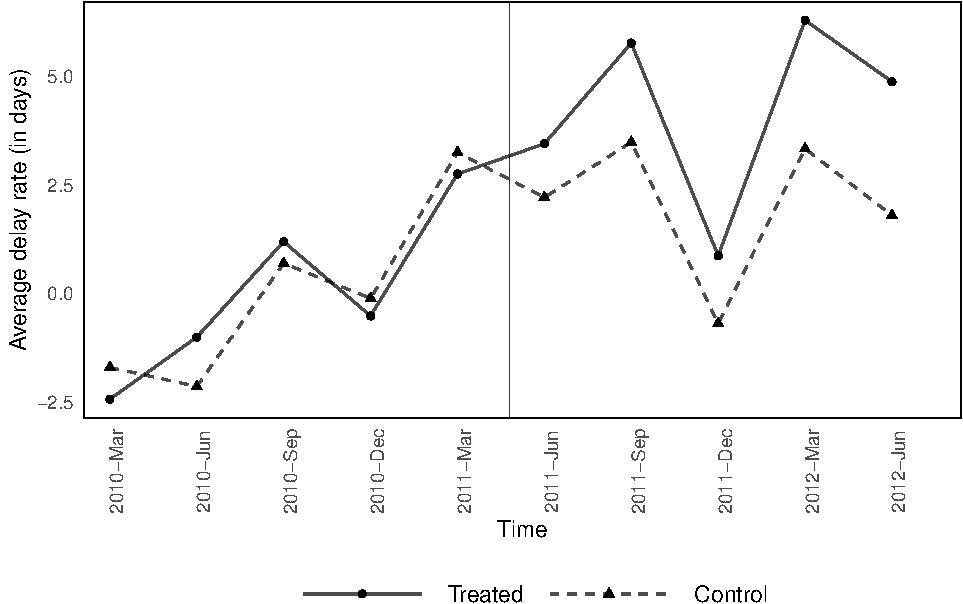
\includegraphics{qp_first_pc_delay-2_files/figure-latex/demeaned_plot_delay_days_one_type-1.pdf}

\hypertarget{percentage-delays-over-time-archived}{%
\section{Percentage delays over time
{[}Archived{]}}\label{percentage-delays-over-time-archived}}

\begin{itemize}
\tightlist
\item
  Sample restricted to projects for which start dates matches the one in
  API

  \begin{itemize}
  \tightlist
  \item
    This is done by using first reported ``action\_date'' and
    ``date\_signed''
  \end{itemize}
\item
  \(PercentDelay_{it}=100 \times Delay_{it}/Duration_{i,t-1}\)

  \begin{itemize}
  \tightlist
  \item
    \(Duration_{i,t-1} = Deadline_{i,t-1} - StartDate_i\)
  \end{itemize}
\end{itemize}

\hypertarget{demeaned-delay-rate-in-percentage-archived}{%
\section{Demeaned delay rate (in percentage)
{[}Archived{]}}\label{demeaned-delay-rate-in-percentage-archived}}

\begin{itemize}
\tightlist
\item
  Subtract the average pre-quickpay delay rate from each observation
\end{itemize}

\hypertarget{demeaned-delay-rate-in-percentage-one-type-contractor}{%
\section{Demeaned delay rate (in percentage) -- One type
contractor}\label{demeaned-delay-rate-in-percentage-one-type-contractor}}

\begin{itemize}
\tightlist
\item
  Subtract the average pre-quickpay delay rate from each observation
\end{itemize}

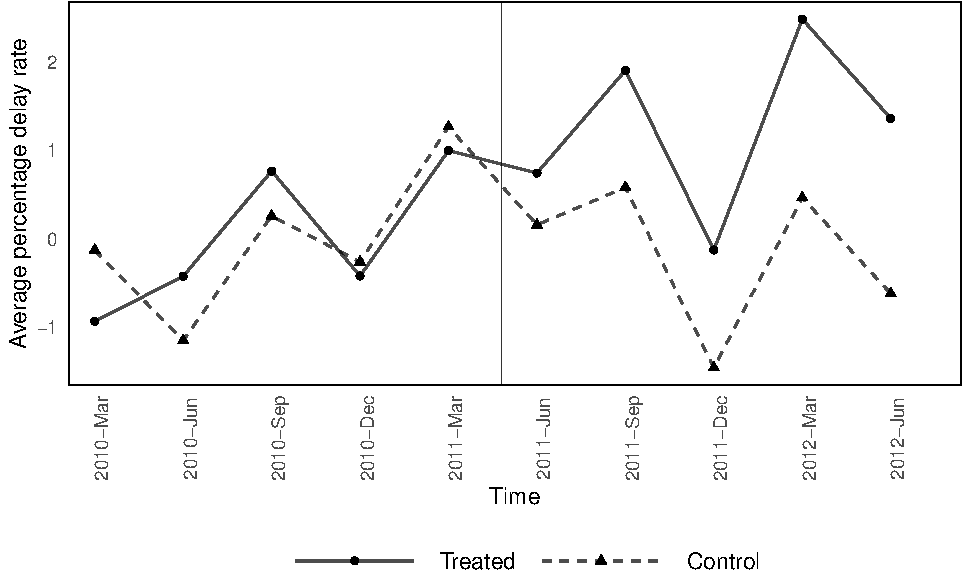
\includegraphics{qp_first_pc_delay-2_files/figure-latex/demeaned_plot_one_type-1.pdf}

\hypertarget{normalized-delay-rate-in-percentage-archived}{%
\section{Normalized delay rate (in percentage)
{[}Archived{]}}\label{normalized-delay-rate-in-percentage-archived}}

\hypertarget{normalized-percentage-delay-four-groups-archived}{%
\section{Normalized percentage delay: Four groups
{[}Archived{]}}\label{normalized-percentage-delay-four-groups-archived}}

\hypertarget{baseline-regressions}{%
\section{Baseline Regressions}\label{baseline-regressions}}

\[ PercentDelay_{it} = \beta_0 + \beta_1 Treat_i + \beta_2 Post_t + \beta_3 (Treat_i \times Post_t) + e_{it}\]

\[ \begin{aligned} PercentDelay_{it} &=& \alpha+\beta_0 Treat_i + \beta_1 Post_t + \beta_2 (Treat_i \times Post_t)\\
&+&  X_i + (Post_t \times X_i) + \mu_t + \theta_{firm} + \lambda_{task}+ \epsilon_{it}
\end{aligned}\]

\begin{table}[H] \centering 
  \caption{Effect of QuickPay on project delay rates} 
  \label{} 
\small 
\begin{tabular}{@{\extracolsep{-2pt}}lccccc} 
\\[-1.8ex]\hline 
\hline \\[-1.8ex] 
\\[-1.8ex] & \multicolumn{5}{c}{$PercentDelay_{it}$} \\ 
\\[-1.8ex] & (1) & (2) & (3) & (4) & (5)\\ 
\hline \\[-1.8ex] 
 $Treat_i$ & $-$2.48$^{***}$ & $-$1.59$^{***}$ & $-$1.62$^{***}$ & $-$1.31$^{***}$ & $-$1.33$^{***}$ \\ 
  & (0.12) & (0.10) & (0.10) & (0.10) & (0.10) \\ 
  & & & & & \\ 
 $Post_t$ & $-$0.32$^{***}$ & $-$8.32$^{***}$ &  &  &  \\ 
  & (0.12) & (0.81) &  &  &  \\ 
  & & & & & \\ 
 $Treat_i \times Post_t$ & 1.27$^{***}$ & 1.10$^{***}$ & 1.13$^{***}$ & 1.18$^{***}$ & 1.23$^{***}$ \\ 
  & (0.14) & (0.13) & (0.13) & (0.13) & (0.13) \\ 
  & & & & & \\ 
 Constant & 6.44$^{***}$ & 53.81$^{***}$ &  &  &  \\ 
  & (0.10) & (0.61) &  &  &  \\ 
  & & & & & \\ 
\hline \\[-1.8ex] 
Duration, Budget, Bids & No & Yes & Yes & Yes & Yes \\ 
$Post_t \times$  (Duration, Budget, Bids) & No & Yes & Yes & Yes & Yes \\ 
Project stage & No & Yes & Yes & Yes & Yes \\ 
Time fixed effects & No & No & Yes & Yes & Yes \\ 
Task fixed effects & No & No & No & Yes & Yes \\ 
Industry fixed effects & No & No & No & No & Yes \\ 
Observations & 260,056 & 235,960 & 235,960 & 235,960 & 235,960 \\ 
R$^{2}$ & 0.003 & 0.22 & 0.22 & 0.25 & 0.26 \\ 
Adjusted R$^{2}$ & 0.003 & 0.22 & 0.22 & 0.25 & 0.25 \\ 
\hline 
\hline \\[-1.8ex] 
\textit{Note:}  & \multicolumn{5}{r}{$^{*}$p$<$0.1; $^{**}$p$<$0.05; $^{***}$p$<$0.01} \\ 
 & \multicolumn{5}{r}{Each observation is a project-quarter.} \\ 
 & \multicolumn{5}{r}{SEs are robust and clustered at the project level.} \\ 
\end{tabular} 
\end{table}

\hypertarget{contractors-performing-only-one-type-of-project-restricted-sample}{%
\subsection{Contractors performing only one type of project (Restricted
sample)}\label{contractors-performing-only-one-type-of-project-restricted-sample}}

\begin{table}[H] \centering 
  \caption{Effect of QuickPay on project delay rates} 
  \label{} 
\small 
\begin{tabular}{@{\extracolsep{-2pt}}lccccc} 
\\[-1.8ex]\hline 
\hline \\[-1.8ex] 
\\[-1.8ex] & \multicolumn{5}{c}{$PercentDelay_{it}$} \\ 
\\[-1.8ex] & (1) & (2) & (3) & (4) & (5)\\ 
\hline \\[-1.8ex] 
 $Treat_i$ & $-$0.94$^{***}$ & $-$0.80$^{***}$ & $-$0.88$^{***}$ & $-$0.89$^{***}$ & $-$0.92$^{***}$ \\ 
  & (0.15) & (0.13) & (0.13) & (0.14) & (0.14) \\ 
  & & & & & \\ 
 $Post_t$ & $-$0.38$^{***}$ & $-$6.94$^{***}$ &  &  &  \\ 
  & (0.14) & (1.06) &  &  &  \\ 
  & & & & & \\ 
 $Treat_i \times Post_t$ & 1.45$^{***}$ & 1.31$^{***}$ & 1.39$^{***}$ & 1.38$^{***}$ & 1.42$^{***}$ \\ 
  & (0.18) & (0.17) & (0.17) & (0.17) & (0.17) \\ 
  & & & & & \\ 
 Constant & 6.12$^{***}$ & 55.77$^{***}$ &  &  &  \\ 
  & (0.11) & (0.81) &  &  &  \\ 
  & & & & & \\ 
\hline \\[-1.8ex] 
Duration, Budget, Bids & No & Yes & Yes & Yes & Yes \\ 
$Post_t \times$  (Duration, Budget, Bids) & No & Yes & Yes & Yes & Yes \\ 
Project stage & No & Yes & Yes & Yes & Yes \\ 
Time fixed effects & No & No & Yes & Yes & Yes \\ 
Task fixed effects & No & No & No & Yes & Yes \\ 
Industry fixed effects & No & No & No & No & Yes \\ 
Observations & 174,197 & 157,166 & 157,166 & 157,166 & 157,166 \\ 
R$^{2}$ & 0.0005 & 0.18 & 0.19 & 0.22 & 0.22 \\ 
Adjusted R$^{2}$ & 0.0005 & 0.18 & 0.18 & 0.21 & 0.21 \\ 
\hline 
\hline \\[-1.8ex] 
\textit{Note:}  & \multicolumn{5}{r}{$^{*}$p$<$0.1; $^{**}$p$<$0.05; $^{***}$p$<$0.01} \\ 
 & \multicolumn{5}{r}{Each observation is a project-quarter.} \\ 
 & \multicolumn{5}{r}{SEs are robust and clustered at the project level.} \\ 
 & \multicolumn{5}{r}{Sample restricted to contractors performing only one type of project.} \\ 
\end{tabular} 
\end{table}

\hypertarget{event-study}{%
\section{Event study}\label{event-study}}

\(PercentDelay_{it}=\beta_0 + \beta_1 Treat_i + \beta_2 Treat_i \times Quarter_t + \gamma_{task} + \theta_{naics}+\lambda_{quarter}+\nu_{sub-agency}+\epsilon_{it}\)

\begin{verbatim}
## NOTE: 242,843 observations removed because of NA values (LHS: 242,843, RHS: 9,862).
\end{verbatim}

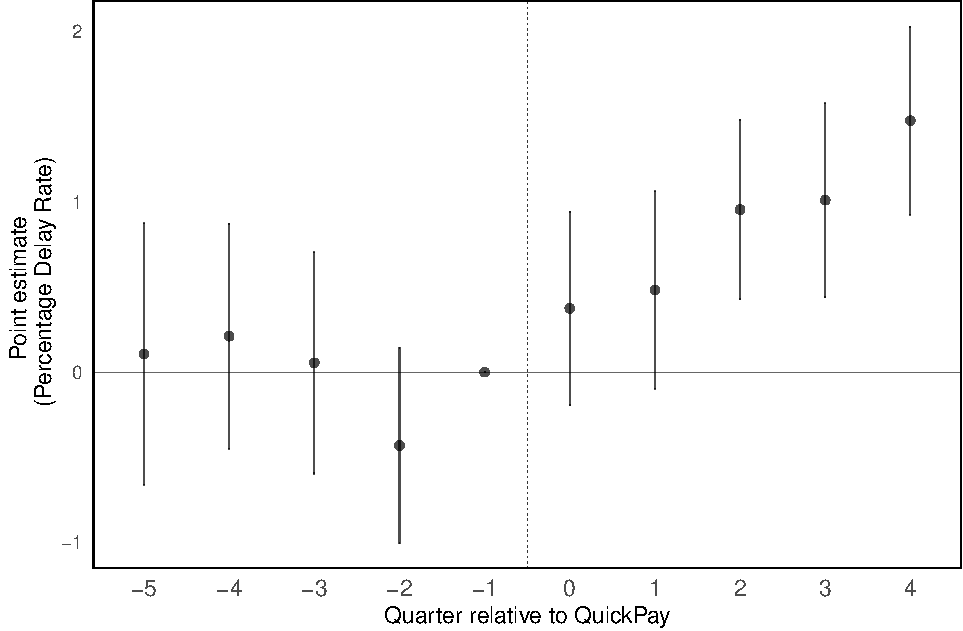
\includegraphics{qp_first_pc_delay-2_files/figure-latex/event_study-1.pdf}

\hypertarget{event-study-one-type}{%
\subsection{Event Study -- One Type}\label{event-study-one-type}}

\begin{verbatim}
## NOTE: 171,267 observations removed because of NA values (LHS: 154,236, RHS: 171,267).
\end{verbatim}

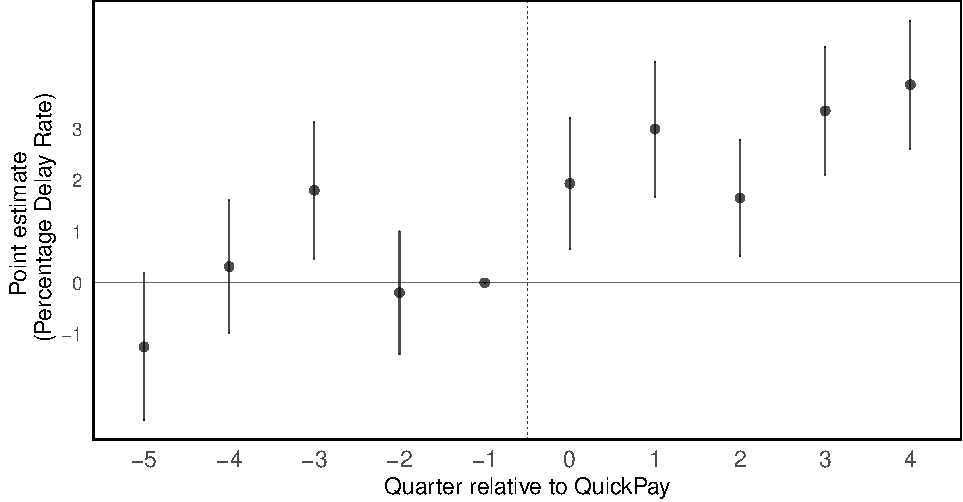
\includegraphics{qp_first_pc_delay-2_files/figure-latex/event_study_one_type-1.pdf}

\hypertarget{parallel-trends-test-one-type}{%
\section{Parallel Trends Test -- One
Type}\label{parallel-trends-test-one-type}}

\begin{table}[H] \centering 
  \caption{Linear Time Trend Before QuickPay} 
  \label{} 
\small 
\begin{tabular}{@{\extracolsep{-2pt}}lccccc} 
\\[-1.8ex]\hline 
\hline \\[-1.8ex] 
\\[-1.8ex] & \multicolumn{5}{c}{$PercentDelay_{it}$} \\ 
\\[-1.8ex] & (1) & (2) & (3) & (4) & (5)\\ 
\hline \\[-1.8ex] 
 $Treat_i$ & $-$0.44 & $-$0.35 & $-$0.34 & $-$0.57 & $-$0.72 \\ 
  & (0.55) & (0.52) & (0.52) & (0.54) & (0.54) \\ 
  & & & & & \\ 
 $QuarterNum$ & 0.47$^{***}$ & $-$1.68$^{**}$ &  &  &  \\ 
  & (0.09) & (0.66) &  &  &  \\ 
  & & & & & \\ 
 $Treat_i \times QuarterNum$ & $-$0.12 & $-$0.13 & $-$0.13 & 0.02 & 0.04 \\ 
  & (0.12) & (0.11) & (0.11) & (0.11) & (0.11) \\ 
  & & & & & \\ 
 Constant & 4.02$^{***}$ & 63.83$^{***}$ &  &  &  \\ 
  & (0.42) & (3.10) &  &  &  \\ 
  & & & & & \\ 
\hline \\[-1.8ex] 
Duration, Budget, Bids & No & Yes & Yes & Yes & Yes \\ 
$Post_t \times$  (Duration, Budget, Bids) & No & Yes & Yes & Yes & Yes \\ 
Project stage & No & Yes & Yes & Yes & Yes \\ 
Time fixed effects & No & No & Yes & Yes & Yes \\ 
Task fixed effects & No & No & No & Yes & Yes \\ 
Industry fixed effects & No & No & No & No & Yes \\ 
Observations & 64,786 & 59,707 & 59,707 & 59,707 & 59,707 \\ 
R$^{2}$ & 0.001 & 0.21 & 0.21 & 0.27 & 0.27 \\ 
Adjusted R$^{2}$ & 0.001 & 0.21 & 0.21 & 0.26 & 0.26 \\ 
\hline 
\hline \\[-1.8ex] 
\textit{Note:}  & \multicolumn{5}{r}{$^{*}$p$<$0.1; $^{**}$p$<$0.05; $^{***}$p$<$0.01} \\ 
 & \multicolumn{5}{r}{Each observation is a project-quarter.} \\ 
 & \multicolumn{5}{r}{SEs are robust and clustered at the project level.} \\ 
 & \multicolumn{5}{r}{Observations are for quarters before quickpay.} \\ 
\end{tabular} 
\end{table}

\hypertarget{placebo-test-one-type}{%
\section{Placebo Test -- One type}\label{placebo-test-one-type}}

\hypertarget{placebo-regression-tables-one-type}{%
\subsection{Placebo Regression Tables -- One
type}\label{placebo-regression-tables-one-type}}

{[}1{]} 4

\begin{table}[H] \centering 
  \caption{Placebo test: Treatment Time 2010-09-30} 
  \label{} 
\small 
\begin{tabular}{@{\extracolsep{-2pt}}lccccc} 
\\[-1.8ex]\hline 
\hline \\[-1.8ex] 
\\[-1.8ex] & \multicolumn{5}{c}{$PercentDelay_{it}$} \\ 
\\[-1.8ex] & (1) & (2) & (3) & (4) & (5)\\ 
\hline \\[-1.8ex] 
 $Treat_i$ & $-$1.03$^{*}$ & $-$2.49$^{***}$ & $-$2.50$^{***}$ & $-$1.51$^{***}$ & $-$1.72$^{***}$ \\ 
  & (0.54) & (0.51) & (0.51) & (0.54) & (0.54) \\ 
  & & & & & \\ 
 $Post$ & 1.81$^{***}$ & $-$13.64$^{***}$ &  &  &  \\ 
  & (0.46) & (3.92) &  &  &  \\ 
  & & & & & \\ 
 $Treat_i \times Post$ & $-$0.95 & 0.50 & 0.48 & 0.61 & 0.71 \\ 
  & (0.61) & (0.59) & (0.59) & (0.59) & (0.59) \\ 
  & & & & & \\ 
 Constant & 8.66$^{***}$ & 112.74$^{***}$ &  &  &  \\ 
  & (0.40) & (3.41) &  &  &  \\ 
  & & & & & \\ 
\hline \\[-1.8ex] 
Duration, Budget, Bids & No & Yes & Yes & Yes & Yes \\ 
$Post_t \times$  (Duration, Budget, Bids) & No & Yes & Yes & Yes & Yes \\ 
Project stage & No & Yes & Yes & Yes & Yes \\ 
Time fixed effects & No & No & Yes & Yes & Yes \\ 
Task fixed effects & No & No & No & Yes & Yes \\ 
Industry fixed effects & No & No & No & No & Yes \\ 
Observations & 64,786 & 59,707 & 59,707 & 59,707 & 59,707 \\ 
R$^{2}$ & 0.001 & 0.22 & 0.22 & 0.27 & 0.28 \\ 
Adjusted R$^{2}$ & 0.001 & 0.22 & 0.22 & 0.26 & 0.26 \\ 
\hline 
\hline \\[-1.8ex] 
\textit{Note:}  & \multicolumn{5}{r}{$^{*}$p$<$0.1; $^{**}$p$<$0.05; $^{***}$p$<$0.01} \\ 
 & \multicolumn{5}{r}{Each observation is a project-quarter.} \\ 
 & \multicolumn{5}{r}{SEs are robust and clustered at the project level.} \\ 
 & \multicolumn{5}{r}{Observations are for quarters before quickpay.} \\ 
\end{tabular} 
\end{table}

{[}1{]} 5

\begin{table}[H] \centering 
  \caption{Placebo test: Treatment Time 2010-12-31} 
  \label{} 
\small 
\begin{tabular}{@{\extracolsep{-2pt}}lccccc} 
\\[-1.8ex]\hline 
\hline \\[-1.8ex] 
\\[-1.8ex] & \multicolumn{5}{c}{$PercentDelay_{it}$} \\ 
\\[-1.8ex] & (1) & (2) & (3) & (4) & (5)\\ 
\hline \\[-1.8ex] 
 $Treat_i$ & $-$1.00$^{**}$ & $-$1.14$^{***}$ & $-$1.18$^{***}$ & $-$0.36 & $-$0.55 \\ 
  & (0.41) & (0.39) & (0.39) & (0.44) & (0.44) \\ 
  & & & & & \\ 
 $Post$ & 1.00$^{**}$ & $-$20.67$^{***}$ &  &  &  \\ 
  & (0.42) & (3.38) &  &  &  \\ 
  & & & & & \\ 
 $Treat_i \times Post$ & $-$1.31$^{**}$ & $-$1.73$^{***}$ & $-$1.66$^{***}$ & $-$1.08$^{**}$ & $-$0.99$^{*}$ \\ 
  & (0.54) & (0.53) & (0.52) & (0.55) & (0.55) \\ 
  & & & & & \\ 
 Constant & 9.48$^{***}$ & 114.18$^{***}$ &  &  &  \\ 
  & (0.31) & (2.60) &  &  &  \\ 
  & & & & & \\ 
\hline \\[-1.8ex] 
Duration, Budget, Bids & No & Yes & Yes & Yes & Yes \\ 
$Post_t \times$  (Duration, Budget, Bids) & No & Yes & Yes & Yes & Yes \\ 
Project stage & No & Yes & Yes & Yes & Yes \\ 
Time fixed effects & No & No & Yes & Yes & Yes \\ 
Task fixed effects & No & No & No & Yes & Yes \\ 
Industry fixed effects & No & No & No & No & Yes \\ 
Observations & 64,786 & 59,707 & 59,707 & 59,707 & 59,707 \\ 
R$^{2}$ & 0.001 & 0.22 & 0.22 & 0.27 & 0.28 \\ 
Adjusted R$^{2}$ & 0.001 & 0.22 & 0.22 & 0.26 & 0.27 \\ 
\hline 
\hline \\[-1.8ex] 
\textit{Note:}  & \multicolumn{5}{r}{$^{*}$p$<$0.1; $^{**}$p$<$0.05; $^{***}$p$<$0.01} \\ 
 & \multicolumn{5}{r}{Each observation is a project-quarter.} \\ 
 & \multicolumn{5}{r}{SEs are robust and clustered at the project level.} \\ 
 & \multicolumn{5}{r}{Observations are for quarters before quickpay.} \\ 
\end{tabular} 
\end{table}

\hypertarget{summary-statistics}{%
\section{Summary statistics}\label{summary-statistics}}

\hypertarget{congestion-effect}{%
\section{Congestion Effect}\label{congestion-effect}}

\hypertarget{number-of-projects-per-contractor}{%
\subsection{Number of projects per
contractor}\label{number-of-projects-per-contractor}}

\hypertarget{contractors-holding-only-small-or-only-large-projects}{%
\subsubsection{Contractors holding only small or only large
projects}\label{contractors-holding-only-small-or-only-large-projects}}

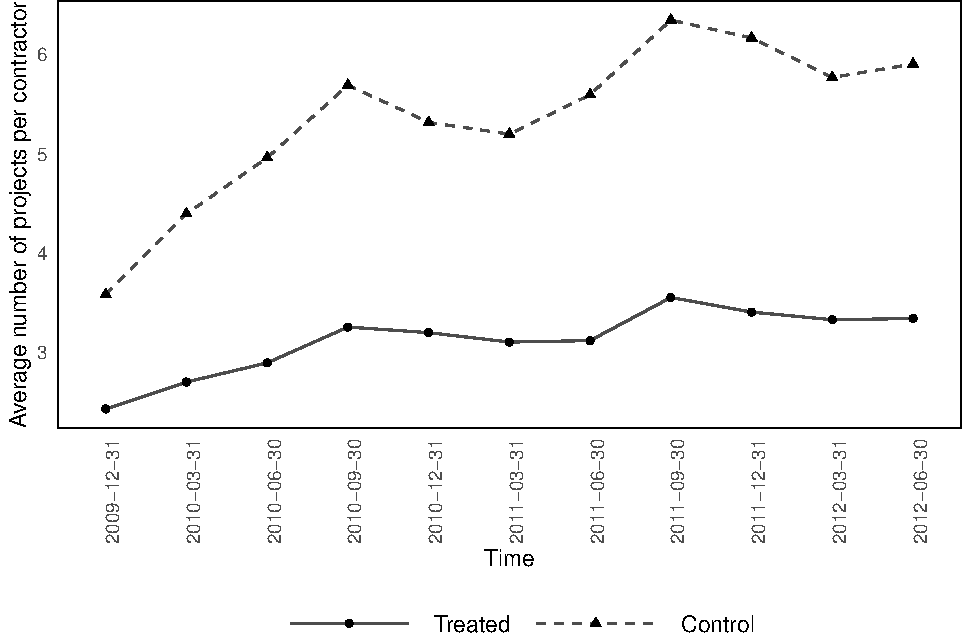
\includegraphics{qp_first_pc_delay-2_files/figure-latex/num_projects_0-1.pdf}

\begin{table}[H] \centering 
  \caption{Num Contractor Projects and QuickPay reform} 
  \label{} 
\small 
\begin{tabular}{@{\extracolsep{-2pt}}lcc} 
\\[-1.8ex]\hline 
\hline \\[-1.8ex] 
\\[-1.8ex] & \multicolumn{2}{c}{Number of projects} \\ 
\\[-1.8ex] & (1) & (2)\\ 
\hline \\[-1.8ex] 
 $Treat_i$ & $-$2.03$^{***}$ & $-$2.03$^{***}$ \\ 
  & (0.39) & (0.39) \\ 
  & & \\ 
 $Post_t$ & 0.94$^{**}$ &  \\ 
  & (0.41) &  \\ 
  & & \\ 
 $Treat_i \times Post_t$ & $-$0.58 & $-$0.58 \\ 
  & (0.41) & (0.41) \\ 
  & & \\ 
 Constant & 5.03$^{***}$ &  \\ 
  & (0.38) &  \\ 
  & & \\ 
\hline \\[-1.8ex] 
Time fixed effects & No & Yes \\ 
Observations & 84,391 & 84,391 \\ 
R$^{2}$ & 0.005 & 0.01 \\ 
Adjusted R$^{2}$ & 0.005 & 0.01 \\ 
\hline 
\hline \\[-1.8ex] 
\textit{Note:}  & \multicolumn{2}{r}{$^{*}$p$<$0.1; $^{**}$p$<$0.05; $^{***}$p$<$0.01} \\ 
 & \multicolumn{2}{r}{Each observation is a contractor-quarter.} \\ 
 & \multicolumn{2}{r}{SEs are robust and clustered at the contractor level.} \\ 
 & \multicolumn{2}{r}{Sample restricted to contractors performing only one type of project.} \\ 
\end{tabular} 
\end{table}

\hypertarget{contractors-holding-at-least-one-small-project-are-treated}{%
\subsubsection{Contractors holding at least one small project are
``treated''}\label{contractors-holding-at-least-one-small-project-are-treated}}

\hypertarget{total-budget}{%
\subsection{Total budget}\label{total-budget}}

\hypertarget{contractors-holding-only-small-or-only-large-projects-1}{%
\subsubsection{Contractors holding only small or only large
projects}\label{contractors-holding-only-small-or-only-large-projects-1}}

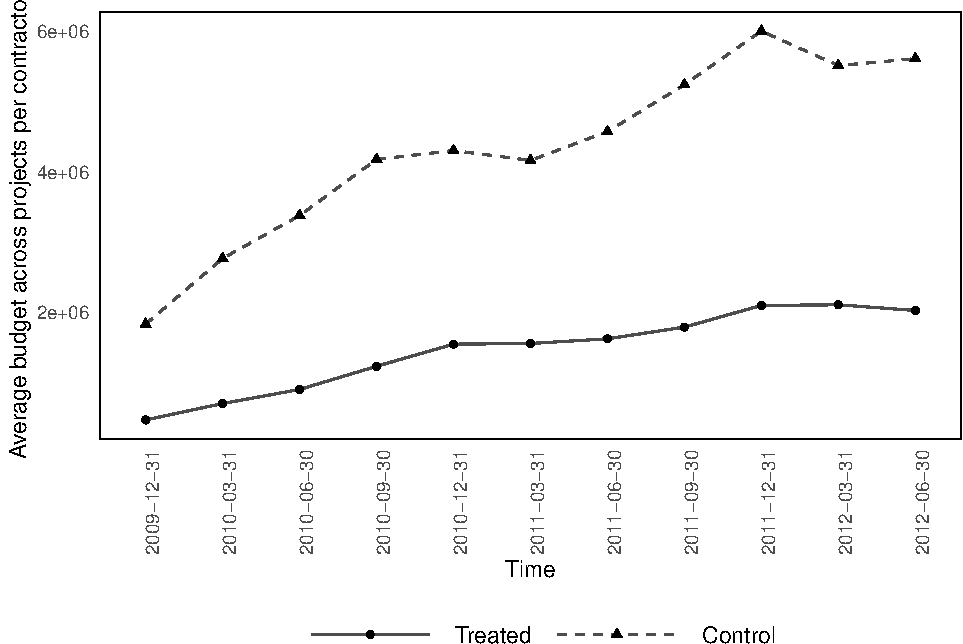
\includegraphics{qp_first_pc_delay-2_files/figure-latex/budget_0-1.pdf}

\begin{table}[H] \centering 
  \caption{Contractor Project Budget and QuickPay reform} 
  \label{} 
\small 
\begin{tabular}{@{\extracolsep{-2pt}}lcc} 
\\[-1.8ex]\hline 
\hline \\[-1.8ex] 
\\[-1.8ex] & \multicolumn{2}{c}{Total budget} \\ 
\\[-1.8ex] & (1) & (2)\\ 
\hline \\[-1.8ex] 
 $Treat_i$ & $-$2,503,033.00$^{***}$ & $-$2,497,737.00$^{***}$ \\ 
  & (454,885.70) & (456,972.80) \\ 
  & & \\ 
 $Post_t$ & 1,715,503.00$^{***}$ &  \\ 
  & (229,333.50) &  \\ 
  & & \\ 
 $Treat_i \times Post_t$ & $-$953,041.30$^{***}$ & $-$955,237.70$^{***}$ \\ 
  & (231,908.60) & (233,131.80) \\ 
  & & \\ 
 Constant & 3,666,740.00$^{***}$ &  \\ 
  & (453,287.80) &  \\ 
  & & \\ 
\hline \\[-1.8ex] 
Time fixed effects & No & Yes \\ 
Observations & 84,391 & 84,391 \\ 
R$^{2}$ & 0.01 & 0.02 \\ 
Adjusted R$^{2}$ & 0.01 & 0.01 \\ 
\hline 
\hline \\[-1.8ex] 
\textit{Note:}  & \multicolumn{2}{r}{$^{*}$p$<$0.1; $^{**}$p$<$0.05; $^{***}$p$<$0.01} \\ 
 & \multicolumn{2}{r}{Each observation is a contractor-quarter.} \\ 
 & \multicolumn{2}{r}{SEs are robust and clustered at the contractor level.} \\ 
 & \multicolumn{2}{r}{Sample restricted to contractors performing only one type of project.} \\ 
\end{tabular} 
\end{table}

\hypertarget{number-of-tasks}{%
\subsection{Number of tasks}\label{number-of-tasks}}

\hypertarget{contractors-holding-only-small-or-only-large-projects-2}{%
\subsubsection{Contractors holding only small or only large
projects}\label{contractors-holding-only-small-or-only-large-projects-2}}

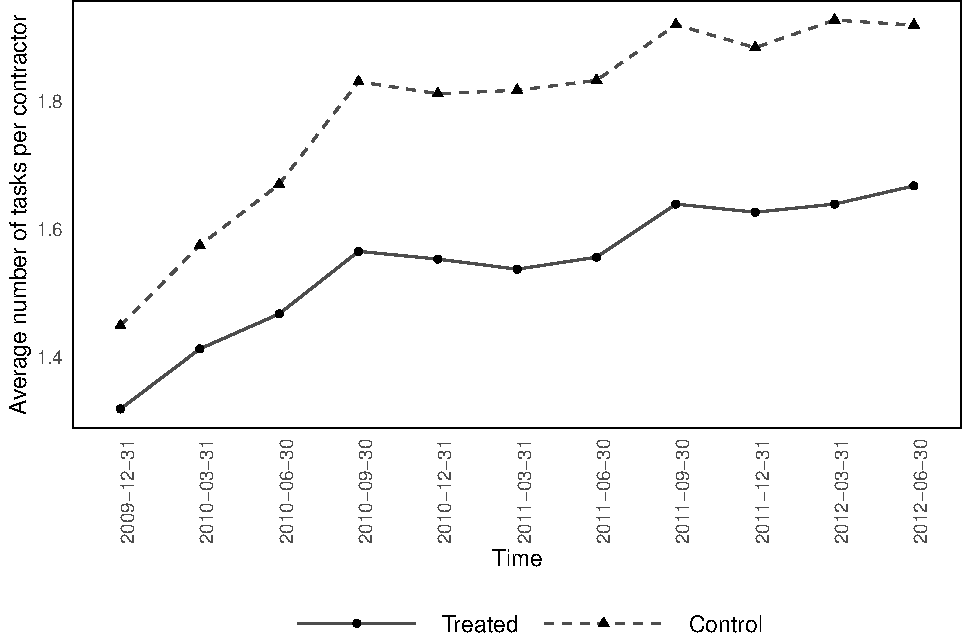
\includegraphics{qp_first_pc_delay-2_files/figure-latex/tasks_0-1.pdf}

\begin{table}[H] \centering 
  \caption{Contractor Project Tasks and QuickPay reform} 
  \label{} 
\small 
\begin{tabular}{@{\extracolsep{-2pt}}lcc} 
\\[-1.8ex]\hline 
\hline \\[-1.8ex] 
\\[-1.8ex] & \multicolumn{2}{c}{Number of tasks} \\ 
\\[-1.8ex] & (1) & (2)\\ 
\hline \\[-1.8ex] 
 $Treat_i$ & $-$0.23$^{***}$ & $-$0.23$^{***}$ \\ 
  & (0.04) & (0.04) \\ 
  & & \\ 
 $Post_t$ & 0.17$^{***}$ &  \\ 
  & (0.02) &  \\ 
  & & \\ 
 $Treat_i \times Post_t$ & $-$0.04 & $-$0.04 \\ 
  & (0.03) & (0.03) \\ 
  & & \\ 
 Constant & 1.73$^{***}$ &  \\ 
  & (0.04) &  \\ 
  & & \\ 
\hline \\[-1.8ex] 
Time fixed effects & No & Yes \\ 
Observations & 84,391 & 84,391 \\ 
R$^{2}$ & 0.01 & 0.01 \\ 
Adjusted R$^{2}$ & 0.01 & 0.01 \\ 
\hline 
\hline \\[-1.8ex] 
\textit{Note:}  & \multicolumn{2}{r}{$^{*}$p$<$0.1; $^{**}$p$<$0.05; $^{***}$p$<$0.01} \\ 
 & \multicolumn{2}{r}{Each observation is a contractor-quarter.} \\ 
 & \multicolumn{2}{r}{SEs are robust and clustered at the contractor level.} \\ 
 & \multicolumn{2}{r}{Sample restricted to contractors performing only one type of project.} \\ 
\end{tabular} 
\end{table}

\hypertarget{project-portfolio-spillover-effect}{%
\section{Project portfolio: Spillover
effect}\label{project-portfolio-spillover-effect}}

\hypertarget{regression-1-did-on-large-projects}{%
\subsection{Regression 1: DID on large
projects}\label{regression-1-did-on-large-projects}}

\begin{itemize}
\tightlist
\item
  Sample restricted to large projects only.
\item
  Treat is an indicator that equals one for LARGE projects that have at
  least one parallel small project in the same quarter, and is zero
  otherwise.
\end{itemize}

\begin{table}[H] \centering 
  \caption{Project Portfolio and QuickPay reform} 
  \label{} 
\small 
\begin{tabular}{@{\extracolsep{-10pt}}lccccc} 
\\[-1.8ex]\hline 
\hline \\[-1.8ex] 
\\[-1.8ex] & \multicolumn{5}{c}{$PercentDelay_{it}$} \\ 
\\[-1.8ex] & (1) & (2) & (3) & (4) & (5)\\ 
\hline \\[-1.8ex] 
 $Treat_i$ & 4.41$^{***}$ & 0.70$^{***}$ & 0.64$^{***}$ & 1.15$^{***}$ & 1.16$^{***}$ \\ 
  & (0.31) & (0.20) & (0.20) & (0.20) & (0.20) \\ 
  & & & & & \\ 
 $Post_t$ & $-$0.10 & $-$13.38$^{***}$ &  &  &  \\ 
  & (0.12) & (1.17) &  &  &  \\ 
  & & & & & \\ 
 $Treat_i \times Post_t$ & $-$1.17$^{***}$ & 0.02 & 0.03 & $-$0.65$^{**}$ & $-$0.56$^{**}$ \\ 
  & (0.36) & (0.26) & (0.26) & (0.26) & (0.26) \\ 
  & & & & & \\ 
 Constant & 5.59$^{***}$ & 63.76$^{***}$ &  &  &  \\ 
  & (0.10) & (0.89) &  &  &  \\ 
  & & & & & \\ 
\hline \\[-1.8ex] 
Duration, Budget, Bids & No & Yes & Yes & Yes & Yes \\ 
$Post_t \times $  (Duration, Budget, Bids) & No & Yes & Yes & Yes & Yes \\ 
Project stage & No & Yes & Yes & Yes & Yes \\ 
Time fixed effects & No & No & Yes & Yes & Yes \\ 
Task fixed effects & No & No & No & Yes & Yes \\ 
Industry fixed effects & No & No & No & No & Yes \\ 
Observations & 117,787 & 110,601 & 110,601 & 110,601 & 110,601 \\ 
R$^{2}$ & 0.01 & 0.26 & 0.26 & 0.30 & 0.30 \\ 
Adjusted R$^{2}$ & 0.01 & 0.26 & 0.26 & 0.29 & 0.29 \\ 
\hline 
\hline \\[-1.8ex] 
\textit{Note:}  & \multicolumn{5}{r}{$^{*}$p$<$0.1; $^{**}$p$<$0.05; $^{***}$p$<$0.01} \\ 
 & \multicolumn{5}{r}{Each observation is a project-quarter.} \\ 
 & \multicolumn{5}{r}{SEs are robust and clustered at the project level.} \\ 
 & \multicolumn{5}{r}{Sample restricted to large projects only.} \\ 
\end{tabular} 
\end{table}

\hypertarget{intensity-with-number-of-small-projects-archived}{%
\subsubsection{Intensity with Number of Small Projects
{[}Archived{]}}\label{intensity-with-number-of-small-projects-archived}}

\hypertarget{regression-2-archived}{%
\subsection{Regression 2 {[}Archived{]}}\label{regression-2-archived}}

\begin{itemize}
\tightlist
\item
  Treat equals one for small projects with at least one large project in
  the same quarter.
\item
  Treat is zero for large projects with NO small project in the same
  quarter.
\item
  Treat is not defined for other cases i.e, only small projects or large
  projects with small projects are excluded.
\end{itemize}

\hypertarget{regression-3-indicator-for-small-project-with-existing-large-project}{%
\subsection{Regression 3: Indicator for small project with existing
large
project}\label{regression-3-indicator-for-small-project-with-existing-large-project}}

\begin{itemize}
\tightlist
\item
  \(Treat_{i,l}\) is an indicator that equals 1 for small projects with
  co-existing large projects, and is zero otherwise.
\item
  \(Treat_{i,l}=1 \implies Treat_i = 1\). This means we have:

  \begin{itemize}
  \tightlist
  \item
    \(Treat_{i,l} \times Post_t = Treat_i \times Treat_{i,l} \times Post_t\)
  \item
    \(Treat_{i,l} \times Treat_i = Treat_{i,l}\)
  \end{itemize}
\item
  Large projects with parallel small projects are removed to get a clean
  control group.
\end{itemize}

\begin{table}[H] \centering 
  \caption{Project Portfolio and QuickPay reform} 
  \label{} 
\small 
\begin{tabular}{@{\extracolsep{-2pt}}lccccc} 
\\[-1.8ex]\hline 
\hline \\[-1.8ex] 
\\[-1.8ex] & \multicolumn{5}{c}{$PercentDelay_{it}$  } \\ 
\\[-1.8ex] & (1) & (2) & (3) & (4) & (5)\\ 
\hline \\[-1.8ex] 
 $Treat_i$ & $-$3.61$^{***}$ & $-$2.45$^{***}$ & $-$2.51$^{***}$ & $-$1.29$^{***}$ & $-$1.26$^{***}$ \\ 
  & (0.15) & (0.15) & (0.15) & (0.15) & (0.15) \\ 
  & & & & & \\ 
 $Treat_{i,l}$ & 2.41$^{***}$ & 1.38$^{***}$ & 1.41$^{***}$ & 0.41$^{***}$ & 0.35$^{***}$ \\ 
  & (0.14) & (0.13) & (0.13) & (0.13) & (0.13) \\ 
  & & & & & \\ 
 $Post_t$ & $-$0.10 & $-$5.88$^{***}$ &  &  &  \\ 
  & (0.12) & (0.88) &  &  &  \\ 
  & & & & & \\ 
 $Treat_i \times Post_t$ & 0.54$^{***}$ & 0.53$^{***}$ & 0.56$^{***}$ & 0.44$^{**}$ & 0.53$^{***}$ \\ 
  & (0.19) & (0.19) & (0.19) & (0.19) & (0.19) \\ 
  & & & & & \\ 
 $Treat_{i,l} \times Post_t$ & 0.67$^{***}$ & 0.66$^{***}$ & 0.65$^{***}$ & 0.68$^{***}$ & 0.62$^{***}$ \\ 
  & (0.17) & (0.18) & (0.17) & (0.17) & (0.17) \\ 
  & & & & & \\ 
 Constant & 5.59$^{***}$ & 48.60$^{***}$ &  &  &  \\ 
  & (0.10) & (0.68) &  &  &  \\ 
  & & & & & \\ 
\hline \\[-1.8ex] 
Duration, Budget, Bids & No & Yes & Yes & Yes & Yes \\ 
$Post_t \times $  (Duration, Budget, Bids) & No & Yes & Yes & Yes & Yes \\ 
Project stage & No & Yes & Yes & Yes & Yes \\ 
Time fixed effects & No & No & Yes & Yes & Yes \\ 
Task fixed effects & No & No & No & Yes & Yes \\ 
Industry fixed effects & No & No & No & No & Yes \\ 
Observations & 237,093 & 214,622 & 214,622 & 214,622 & 214,622 \\ 
R$^{2}$ & 0.004 & 0.18 & 0.18 & 0.21 & 0.21 \\ 
Adjusted R$^{2}$ & 0.004 & 0.18 & 0.18 & 0.21 & 0.21 \\ 
\hline 
\hline \\[-1.8ex] 
\textit{Note:}  & \multicolumn{5}{r}{$^{*}$p$<$0.1; $^{**}$p$<$0.05; $^{***}$p$<$0.01} \\ 
 & \multicolumn{5}{r}{Each observation is a project-quarter.} \\ 
 & \multicolumn{5}{r}{SEs are robust and clustered at the project level.} \\ 
 & \multicolumn{5}{r}{Large projects with parallel small projects are removed.} \\ 
\end{tabular} 
\end{table}

\hypertarget{regression-4a-indicator-for-parallel-large-project-archived}{%
\subsection{Regression 4A: Indicator for Parallel Large Project
{[}Archived{]}}\label{regression-4a-indicator-for-parallel-large-project-archived}}

\begin{itemize}
\tightlist
\item
  Concurrent Large Project\(_{i,t}\) is an indicator that equals one if
  the contractor has at least one other large project in the same
  quarter.
\item
  Large projects with parallel small projects are removed to get a clean
  control group.
\end{itemize}

\hypertarget{regression-4b-number-of-large-projects-archived}{%
\subsection{Regression 4B: Number of Large Projects
{[}Archived{]}}\label{regression-4b-number-of-large-projects-archived}}

\hypertarget{archived-mediator-total-projects}{%
\subsubsection{{[}ARCHIVED{]} Mediator: Total
Projects}\label{archived-mediator-total-projects}}

\hypertarget{archived-project-portfolio-num-large-projectstotal-projects}{%
\section{{[}Archived{]} Project portfolio: Num Large Projects/Total
Projects}\label{archived-project-portfolio-num-large-projectstotal-projects}}

\hypertarget{continuous}{%
\subsection{Continuous}\label{continuous}}

\hypertarget{total-number-of-projects}{%
\subsubsection{Total Number of
Projects}\label{total-number-of-projects}}

\hypertarget{discrete}{%
\subsection{Discrete}\label{discrete}}

\hypertarget{pre-defined-proportions}{%
\subsubsection{Pre-defined proportions}\label{pre-defined-proportions}}

\hypertarget{proportions-based-on-quintiles}{%
\subsubsection{Proportions based on
Quintiles}\label{proportions-based-on-quintiles}}

\hypertarget{archived-project-portfolio-budget-large-projectstotal-budget-across-projects}{%
\section{{[}Archived{]} Project portfolio: Budget Large Projects/Total
Budget Across
Projects}\label{archived-project-portfolio-budget-large-projectstotal-budget-across-projects}}

\hypertarget{project-stage}{%
\section{Project Stage}\label{project-stage}}

\begin{itemize}
\tightlist
\item
  \(t\) indicates the end of the quarter
\item
  We want to get stage of the project at the beginning of a given
  quarter (before any delays materialize)
\end{itemize}

\(Stage_{it}=\frac{ActionDate_{t-1}-StartDate_i}{Duration_{i,t-1}}\)
\(Stage_{it}=\frac{(t-1)-StartDate_i}{Duration_{i,t-1}}\)

\begin{table}[H] \centering 
  \caption{Project Stage and QuickPay reform} 
  \label{} 
\small 
\begin{tabular}{@{\extracolsep{-2pt}}lccccc} 
\\[-1.8ex]\hline 
\hline \\[-1.8ex] 
\\[-1.8ex] & \multicolumn{5}{c}{$PercentDelay_{it}$  } \\ 
\\[-1.8ex] & (1) & (2) & (3) & (4) & (5)\\ 
\hline \\[-1.8ex] 
 $Treat_i$ & $-$0.40$^{***}$ & $-$1.21$^{***}$ & $-$1.18$^{***}$ & $-$0.88$^{***}$ & $-$0.87$^{***}$ \\ 
  & (0.09) & (0.11) & (0.11) & (0.12) & (0.12) \\ 
  & & & & & \\ 
 Medium Stage & 0.93$^{***}$ & 0.52$^{***}$ & 0.38$^{***}$ & 0.69$^{***}$ & 0.68$^{***}$ \\ 
  & (0.12) & (0.13) & (0.13) & (0.13) & (0.13) \\ 
  & & & & & \\ 
 Late Stage & 16.93$^{***}$ & 11.90$^{***}$ & 11.75$^{***}$ & 11.42$^{***}$ & 11.40$^{***}$ \\ 
  & (0.28) & (0.23) & (0.23) & (0.23) & (0.23) \\ 
  & & & & & \\ 
 $Post_t$ & $-$0.15 & $-$6.48$^{***}$ &  &  &  \\ 
  & (0.09) & (0.79) &  &  &  \\ 
  & & & & & \\ 
 $Treat_i \times Post_t$ & 0.19$^{*}$ & 0.10 & 0.09 & 0.08 & 0.13 \\ 
  & (0.12) & (0.15) & (0.15) & (0.15) & (0.15) \\ 
  & & & & & \\ 
 $Treat_i \times$ Medium Stage & $-$0.48$^{***}$ & 0.32$^{**}$ & 0.30$^{*}$ & 0.24 & 0.24 \\ 
  & (0.15) & (0.16) & (0.16) & (0.16) & (0.16) \\ 
  & & & & & \\ 
 $Treat_i \times$ Late Stage & $-$5.01$^{***}$ & $-$1.68$^{***}$ & $-$1.75$^{***}$ & $-$1.88$^{***}$ & $-$1.96$^{***}$ \\ 
  & (0.36) & (0.31) & (0.31) & (0.30) & (0.30) \\ 
  & & & & & \\ 
 $Post_t \times$ Medium Stage & $-$0.80$^{***}$ & 0.37$^{**}$ & 0.25 & $-$0.04 & $-$0.05 \\ 
  & (0.15) & (0.16) & (0.16) & (0.16) & (0.16) \\ 
  & & & & & \\ 
 $Post_t \times$ Late Stage & $-$5.50$^{***}$ & $-$1.93$^{***}$ & $-$1.99$^{***}$ & $-$2.45$^{***}$ & $-$2.46$^{***}$ \\ 
  & (0.32) & (0.27) & (0.27) & (0.27) & (0.27) \\ 
  & & & & & \\ 
 $Treat_i \times Post_t \times$ Medium Stage & 0.39$^{**}$ & $-$0.01 & $-$0.02 & 0.15 & 0.15 \\ 
  & (0.18) & (0.21) & (0.21) & (0.20) & (0.20) \\ 
  & & & & & \\ 
 $Treat_i \times Post_t \times$ Late Stage & 3.80$^{***}$ & 2.81$^{***}$ & 2.86$^{***}$ & 3.04$^{***}$ & 3.09$^{***}$ \\ 
  & (0.41) & (0.37) & (0.37) & (0.36) & (0.36) \\ 
  & & & & & \\ 
 Constant & 1.51$^{***}$ & 44.16$^{***}$ &  &  &  \\ 
  & (0.07) & (0.60) &  &  &  \\ 
  & & & & & \\ 
\hline \\[-1.8ex] 
Duration, Budget, Bids & No & Yes & Yes & Yes & Yes \\ 
$Post_t \times $  (Duration, Budget, Bids) & No & Yes & Yes & Yes & Yes \\ 
Time fixed effects & No & No & Yes & Yes & Yes \\ 
Task fixed effects & No & No & No & Yes & Yes \\ 
Industry fixed effects & No & No & No & No & Yes \\ 
Observations & 260,000 & 235,960 & 235,960 & 235,960 & 235,960 \\ 
R$^{2}$ & 0.11 & 0.24 & 0.24 & 0.27 & 0.27 \\ 
Adjusted R$^{2}$ & 0.11 & 0.24 & 0.24 & 0.27 & 0.27 \\ 
\hline 
\hline \\[-1.8ex] 
\textit{Note:}  & \multicolumn{5}{r}{$^{*}$p$<$0.1; $^{**}$p$<$0.05; $^{***}$p$<$0.01} \\ 
 & \multicolumn{5}{r}{Each observation is a project-quarter.} \\ 
 & \multicolumn{5}{r}{SEs are robust and clustered at the project level.} \\ 
\end{tabular} 
\end{table}

\hypertarget{stage-decile-regression-plots}{%
\subsection{Stage decile Regression
Plots}\label{stage-decile-regression-plots}}

\hypertarget{stage-quintile}{%
\subsection{Stage Quintile}\label{stage-quintile}}

\hypertarget{logged-stage-regressions}{%
\subsection{Logged Stage Regressions}\label{logged-stage-regressions}}

\begin{table}[H] \centering 
  \caption{Project Stage and QuickPay reform} 
  \label{} 
\small 
\begin{tabular}{@{\extracolsep{-2pt}}lccccc} 
\\[-1.8ex]\hline 
\hline \\[-1.8ex] 
\\[-1.8ex] & \multicolumn{5}{c}{$PercentDelay_{it}$  } \\ 
\\[-1.8ex] & (1) & (2) & (3) & (4) & (5)\\ 
\hline \\[-1.8ex] 
 $Treat_i$ & $-$4.72$^{***}$ & $-$2.45$^{***}$ & $-$2.50$^{***}$ & $-$2.14$^{***}$ & $-$2.19$^{***}$ \\ 
  & (0.25) & (0.21) & (0.21) & (0.20) & (0.20) \\ 
  & & & & & \\ 
 Log(Stage) & 4.50$^{***}$ & 3.17$^{***}$ & 3.12$^{***}$ & 3.14$^{***}$ & 3.14$^{***}$ \\ 
  & (0.08) & (0.07) & (0.07) & (0.07) & (0.07) \\ 
  & & & & & \\ 
 $Post_t$ & $-$2.20$^{***}$ & $-$7.92$^{***}$ &  &  &  \\ 
  & (0.23) & (0.83) &  &  &  \\ 
  & & & & & \\ 
 $Treat_i \times Post_t$ & 2.88$^{***}$ & 2.10$^{***}$ & 2.14$^{***}$ & 2.25$^{***}$ & 2.33$^{***}$ \\ 
  & (0.30) & (0.26) & (0.26) & (0.25) & (0.25) \\ 
  & & & & & \\ 
 $Treat_i \times$ Log(Stage) & $-$1.65$^{***}$ & $-$0.54$^{***}$ & $-$0.55$^{***}$ & $-$0.52$^{***}$ & $-$0.55$^{***}$ \\ 
  & (0.11) & (0.09) & (0.09) & (0.09) & (0.09) \\ 
  & & & & & \\ 
 $Post_t \times$ Log(Stage) & $-$0.36$^{***}$ & 0.53$^{***}$ & 0.53$^{***}$ & 0.23$^{***}$ & 0.22$^{**}$ \\ 
  & (0.10) & (0.09) & (0.09) & (0.09) & (0.09) \\ 
  & & & & & \\ 
 $Treat_i \times Post_t \times$ Log(Stage) & 0.93$^{***}$ & 0.64$^{***}$ & 0.65$^{***}$ & 0.71$^{***}$ & 0.73$^{***}$ \\ 
  & (0.13) & (0.12) & (0.12) & (0.12) & (0.12) \\ 
  & & & & & \\ 
 Constant & 13.35$^{***}$ & 53.91$^{***}$ &  &  &  \\ 
  & (0.20) & (0.62) &  &  &  \\ 
  & & & & & \\ 
\hline \\[-1.8ex] 
Duration, Budget, Bids & No & Yes & Yes & Yes & Yes \\ 
$Post_t \times $  (Duration, Budget, Bids) & No & Yes & Yes & Yes & Yes \\ 
Time fixed effects & No & No & Yes & Yes & Yes \\ 
Task fixed effects & No & No & No & Yes & Yes \\ 
Industry fixed effects & No & No & No & No & Yes \\ 
Observations & 260,000 & 235,960 & 235,960 & 235,960 & 235,960 \\ 
R$^{2}$ & 0.06 & 0.22 & 0.22 & 0.25 & 0.26 \\ 
Adjusted R$^{2}$ & 0.06 & 0.22 & 0.22 & 0.25 & 0.25 \\ 
\hline 
\hline \\[-1.8ex] 
\textit{Note:}  & \multicolumn{5}{r}{$^{*}$p$<$0.1; $^{**}$p$<$0.05; $^{***}$p$<$0.01} \\ 
 & \multicolumn{5}{r}{Each observation is a project-quarter.} \\ 
 & \multicolumn{5}{r}{SEs are robust and clustered at the project level.} \\ 
\end{tabular} 
\end{table}

\hypertarget{restricted-sample-one-type}{%
\subsubsection{Restricted sample: One
type}\label{restricted-sample-one-type}}

\begin{table}[H] \centering 
  \caption{Project Stage and QuickPay reform} 
  \label{} 
\small 
\begin{tabular}{@{\extracolsep{-2pt}}lccccc} 
\\[-1.8ex]\hline 
\hline \\[-1.8ex] 
\\[-1.8ex] & \multicolumn{5}{c}{$PercentDelay_{it}$  } \\ 
\\[-1.8ex] & (1) & (2) & (3) & (4) & (5)\\ 
\hline \\[-1.8ex] 
 $Treat_i$ & $-$0.93$^{***}$ & $-$0.44$^{*}$ & $-$0.58$^{**}$ & $-$0.66$^{**}$ & $-$0.73$^{***}$ \\ 
  & (0.31) & (0.27) & (0.27) & (0.27) & (0.27) \\ 
  & & & & & \\ 
 Log(Stage) & 3.70$^{***}$ & 2.86$^{***}$ & 2.81$^{***}$ & 2.92$^{***}$ & 2.93$^{***}$ \\ 
  & (0.09) & (0.09) & (0.09) & (0.09) & (0.09) \\ 
  & & & & & \\ 
 $Post_t$ & $-$1.81$^{***}$ & $-$6.40$^{***}$ &  &  &  \\ 
  & (0.27) & (1.08) &  &  &  \\ 
  & & & & & \\ 
 $Treat_i \times Post_t$ & 2.09$^{***}$ & 2.11$^{***}$ & 2.22$^{***}$ & 2.35$^{***}$ & 2.41$^{***}$ \\ 
  & (0.36) & (0.33) & (0.33) & (0.33) & (0.33) \\ 
  & & & & & \\ 
 $Treat_i \times$ Log(Stage) & $-$0.23$^{*}$ & 0.26$^{**}$ & 0.22$^{*}$ & 0.16 & 0.13 \\ 
  & (0.12) & (0.12) & (0.12) & (0.12) & (0.11) \\ 
  & & & & & \\ 
 $Post_t \times$ Log(Stage) & $-$0.15 & 0.56$^{***}$ & 0.56$^{***}$ & 0.24$^{**}$ & 0.23$^{**}$ \\ 
  & (0.11) & (0.11) & (0.11) & (0.11) & (0.11) \\ 
  & & & & & \\ 
 $Treat_i \times Post_t \times$ Log(Stage) & 0.65$^{***}$ & 0.68$^{***}$ & 0.70$^{***}$ & 0.83$^{***}$ & 0.84$^{***}$ \\ 
  & (0.16) & (0.15) & (0.15) & (0.15) & (0.15) \\ 
  & & & & & \\ 
 Constant & 11.91$^{***}$ & 55.41$^{***}$ &  &  &  \\ 
  & (0.23) & (0.82) &  &  &  \\ 
  & & & & & \\ 
\hline \\[-1.8ex] 
Duration, Budget, Bids & No & Yes & Yes & Yes & Yes \\ 
$Post_t \times $  (Duration, Budget, Bids) & No & Yes & Yes & Yes & Yes \\ 
Time fixed effects & No & No & Yes & Yes & Yes \\ 
Task fixed effects & No & No & No & Yes & Yes \\ 
Industry fixed effects & No & No & No & No & Yes \\ 
Observations & 174,169 & 157,166 & 157,166 & 157,166 & 157,166 \\ 
R$^{2}$ & 0.06 & 0.19 & 0.19 & 0.22 & 0.22 \\ 
Adjusted R$^{2}$ & 0.06 & 0.19 & 0.19 & 0.21 & 0.21 \\ 
\hline 
\hline \\[-1.8ex] 
\textit{Note:}  & \multicolumn{5}{r}{$^{*}$p$<$0.1; $^{**}$p$<$0.05; $^{***}$p$<$0.01} \\ 
 & \multicolumn{5}{r}{Each observation is a project-quarter.} \\ 
 & \multicolumn{5}{r}{SEs are robust and clustered at the project level.} \\ 
 & \multicolumn{5}{r}{Sample restricted to contractors holding only one type of project.} \\ 
\end{tabular} 
\end{table}

\hypertarget{stage-quintile-one-type}{%
\subsection{Stage Quintile -- One Type}\label{stage-quintile-one-type}}

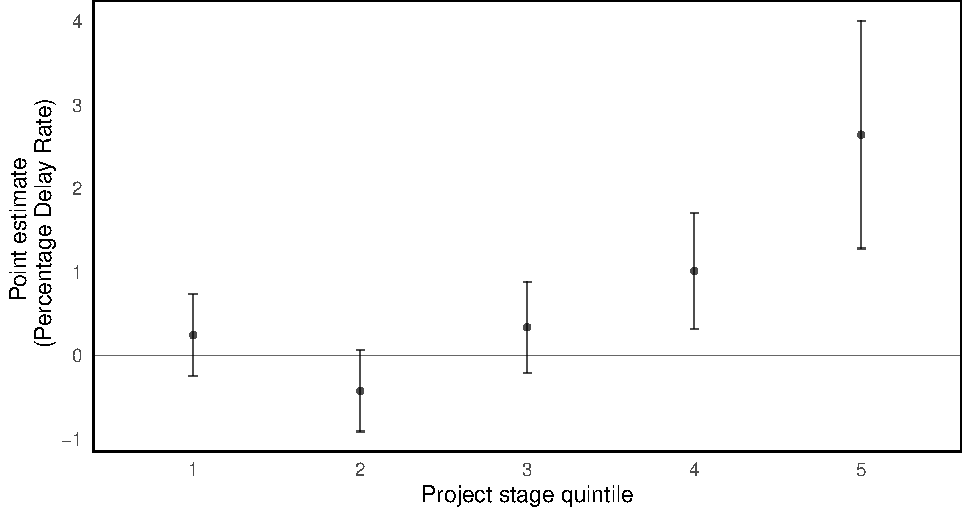
\includegraphics{qp_first_pc_delay-2_files/figure-latex/stage_quintile_one_type-1.pdf}
stage\_quintile Min stage Max stage 1: 1 0.00 0.11 2: 2 0.11 0.27 3: 3
0.27 0.45 4: 4 0.45 0.66 5: 5 0.66 1.00

\hypertarget{aliter-stage-definition-archived}{%
\subsection{Aliter: Stage definition
{[}Archived{]}}\label{aliter-stage-definition-archived}}

\begin{itemize}
\tightlist
\item
  \(t\) indicates the end of the quarter
\end{itemize}

\(Stage_{it}=\frac{ActionDate_{t}-StartDate_i}{Duration_{i,t}}\)
\(Stage_{it}=\frac{t-StartDate_i}{Duration_{i,t}}\)

\hypertarget{contract-financing-archived}{%
\section{Contract Financing
{[}Archived{]}}\label{contract-financing-archived}}

\[ CF_i = \begin{cases} 1, \text{ if project } i \text{ receives contract financing}\\
0, \text{ otherwise} \end{cases}\]

\[ \begin{aligned}
PercentDelay_{it} &=& \beta_0+\beta_1 Treat_i + \beta_2 Post_t + \beta_3 (Treat_i \times Post_t) \\
&+&\beta_4 CF_i + \beta_5 (CF_i \times Post_t) + \beta_6 (Treat_i \times Post_t \times CF_i) \\ 
&+&X_i + (Post_t \times X_i) + \mu_t + \theta_{firm} + \lambda_{task}+ \epsilon_{it}
\end{aligned}\]

\hypertarget{with-treat-x-cf-term}{%
\subsection{With Treat x CF term}\label{with-treat-x-cf-term}}

\hypertarget{projects-active-onbefore-june-2010}{%
\subsection{Projects active on/before June
2010}\label{projects-active-onbefore-june-2010}}

\begin{itemize}
\tightlist
\item
  \(CF=1\) if project was receiving contract financing
\item
  Sample restricted to projects that started on or before June 2010
\item
  Jobs act was launched in Sept 2010
\end{itemize}

\hypertarget{firm-level-financial-constraints-onbefore-june-2010}{%
\subsection{Firm level financial Constraints (on/before June
2010)}\label{firm-level-financial-constraints-onbefore-june-2010}}

\begin{itemize}
\tightlist
\item
  \(CF=1\) if contractor was receiving financing on any project prior on
  or before June 2010
\item
  Jobs act was launched in Sept 2010
\end{itemize}

\hypertarget{plots}{%
\subsection{Plots}\label{plots}}

\hypertarget{receives-grantsfinancial-assistance}{%
\section{Receives Grants/Financial
Assistance}\label{receives-grantsfinancial-assistance}}

\begin{itemize}
\tightlist
\item
  \(CF=1\) if receives\_grants==`t'
\item
  The variable ``receives\_grants'' used to be called ``receives
  financial assistance''
\end{itemize}

\hypertarget{all-projects-archived}{%
\subsection{All projects {[}Archived{]}}\label{all-projects-archived}}

\hypertarget{projects-active-onbefore-june-2010-1}{%
\subsection{Projects active on/before June
2010}\label{projects-active-onbefore-june-2010-1}}

\begin{table}[H] \centering 
  \caption{Financial constraints and QuickPay reform} 
  \label{} 
\small 
\begin{tabular}{@{\extracolsep{-2pt}}lccccc} 
\\[-1.8ex]\hline 
\hline \\[-1.8ex] 
\\[-1.8ex] & \multicolumn{5}{c}{$PercentDelay_{it}$  } \\ 
\\[-1.8ex] & (1) & (2) & (3) & (4) & (5)\\ 
\hline \\[-1.8ex] 
 $Treat_i$ & $-$2.14$^{***}$ & $-$1.08$^{***}$ & $-$1.17$^{***}$ & $-$0.67$^{***}$ & $-$0.74$^{***}$ \\ 
  & (0.15) & (0.14) & (0.14) & (0.14) & (0.14) \\ 
  & & & & & \\ 
 $Post_t$ & 1.90$^{***}$ & $-$17.47$^{***}$ &  &  &  \\ 
  & (0.26) & (2.36) &  &  &  \\ 
  & & & & & \\ 
 $CF_i$ & 13.75$^{***}$ & 6.69$^{***}$ & 6.18$^{***}$ & 4.62$^{***}$ & 4.67$^{***}$ \\ 
  & (1.00) & (0.58) & (0.58) & (0.59) & (0.59) \\ 
  & & & & & \\ 
 $Treat_i \times Post_t$ & $-$0.24 & 1.97$^{***}$ & 2.05$^{***}$ & 2.19$^{***}$ & 2.17$^{***}$ \\ 
  & (0.33) & (0.41) & (0.41) & (0.42) & (0.42) \\ 
  & & & & & \\ 
 $Post_t \times CF_i$ & $-$9.66$^{***}$ & $-$7.56$^{***}$ & $-$6.98$^{***}$ & $-$5.33$^{***}$ & $-$5.28$^{***}$ \\ 
  & (1.29) & (1.28) & (1.27) & (1.29) & (1.28) \\ 
  & & & & & \\ 
 $Treat_i \times CF_i$ & $-$10.08$^{***}$ & $-$2.88$^{***}$ & $-$2.50$^{***}$ & $-$2.83$^{***}$ & $-$2.91$^{***}$ \\ 
  & (1.18) & (0.81) & (0.80) & (0.80) & (0.81) \\ 
  & & & & & \\ 
 $Treat_i \times Post_t \times CF_i$ & 8.20$^{***}$ & 5.50$^{***}$ & 5.12$^{***}$ & 5.21$^{***}$ & 5.42$^{***}$ \\ 
  & (1.62) & (1.83) & (1.82) & (1.84) & (1.83) \\ 
  & & & & & \\ 
 Constant & 6.03$^{***}$ & 56.28$^{***}$ &  &  &  \\ 
  & (0.13) & (0.83) &  &  &  \\ 
  & & & & & \\ 
\hline \\[-1.8ex] 
Duration, Budget, Bids & No & Yes & Yes & Yes & Yes \\ 
$Post_t \times $  (Duration, Budget, Bids) & No & Yes & Yes & Yes & Yes \\ 
Project stage & No & Yes & Yes & Yes & Yes \\ 
Time fixed effects & No & No & Yes & Yes & Yes \\ 
Task fixed effects & No & No & No & Yes & Yes \\ 
Industry fixed effects & No & No & No & No & Yes \\ 
Observations & 75,119 & 64,292 & 64,292 & 64,292 & 64,292 \\ 
R$^{2}$ & 0.02 & 0.23 & 0.23 & 0.27 & 0.28 \\ 
Adjusted R$^{2}$ & 0.02 & 0.23 & 0.23 & 0.26 & 0.27 \\ 
\hline 
\hline \\[-1.8ex] 
\textit{Note:}  & \multicolumn{5}{r}{$^{*}$p$<$0.1; $^{**}$p$<$0.05; $^{***}$p$<$0.01} \\ 
 & \multicolumn{5}{r}{Each observation is a project-quarter.} \\ 
 & \multicolumn{5}{r}{SEs are robust and clustered at the project level.} \\ 
\end{tabular} 
\end{table}

\hypertarget{projects-active-onbefore-june-2010-one-type}{%
\subsection{Projects active on/before June 2010 -- One
type}\label{projects-active-onbefore-june-2010-one-type}}

\begin{table}[H] \centering 
  \caption{Financial constraints and QuickPay reform} 
  \label{} 
\small 
\begin{tabular}{@{\extracolsep{-2pt}}lccccc} 
\\[-1.8ex]\hline 
\hline \\[-1.8ex] 
\\[-1.8ex] & \multicolumn{5}{c}{$PercentDelay_{it}$  } \\ 
\\[-1.8ex] & (1) & (2) & (3) & (4) & (5)\\ 
\hline \\[-1.8ex] 
 $Treat_i$ & $-$1.18$^{***}$ & $-$0.33$^{*}$ & $-$0.51$^{***}$ & $-$0.27 & $-$0.37$^{*}$ \\ 
  & (0.20) & (0.18) & (0.18) & (0.21) & (0.21) \\ 
  & & & & & \\ 
 $Post_t$ & 1.34$^{***}$ & $-$13.60$^{***}$ &  &  &  \\ 
  & (0.30) & (3.40) &  &  &  \\ 
  & & & & & \\ 
 $CF_i$ & 0.74 & 2.34$^{***}$ & 2.06$^{**}$ & 1.61$^{**}$ & 1.63$^{**}$ \\ 
  & (0.90) & (0.83) & (0.82) & (0.80) & (0.80) \\ 
  & & & & & \\ 
 $Treat_i \times Post_t$ & $-$0.50 & 1.97$^{***}$ & 2.15$^{***}$ & 2.56$^{***}$ & 2.56$^{***}$ \\ 
  & (0.38) & (0.48) & (0.48) & (0.50) & (0.50) \\ 
  & & & & & \\ 
 $Post_t \times CF_i$ & $-$1.06 & $-$2.06 & $-$1.70 & $-$0.43 & $-$0.35 \\ 
  & (1.33) & (1.59) & (1.58) & (1.65) & (1.64) \\ 
  & & & & & \\ 
 $Treat_i \times CF_i$ & 2.78$^{**}$ & 1.29 & 1.44 & 0.38 & 0.42 \\ 
  & (1.19) & (1.06) & (1.05) & (1.04) & (1.05) \\ 
  & & & & & \\ 
 $Treat_i \times Post_t \times CF_i$ & $-$0.06 & 0.47 & 0.33 & 0.63 & 0.78 \\ 
  & (1.77) & (2.18) & (2.17) & (2.23) & (2.22) \\ 
  & & & & & \\ 
 Constant & 6.38$^{***}$ & 59.58$^{***}$ &  &  &  \\ 
  & (0.15) & (1.10) &  &  &  \\ 
  & & & & & \\ 
\hline \\[-1.8ex] 
Duration, Budget, Bids & No & Yes & Yes & Yes & Yes \\ 
$Post_t \times $  (Duration, Budget, Bids) & No & Yes & Yes & Yes & Yes \\ 
Project stage & No & Yes & Yes & Yes & Yes \\ 
Time fixed effects & No & No & Yes & Yes & Yes \\ 
Task fixed effects & No & No & No & Yes & Yes \\ 
Industry fixed effects & No & No & No & No & Yes \\ 
Observations & 51,465 & 43,519 & 43,519 & 43,519 & 43,519 \\ 
R$^{2}$ & 0.002 & 0.18 & 0.19 & 0.23 & 0.24 \\ 
Adjusted R$^{2}$ & 0.002 & 0.18 & 0.19 & 0.22 & 0.22 \\ 
\hline 
\hline \\[-1.8ex] 
\textit{Note:}  & \multicolumn{5}{r}{$^{*}$p$<$0.1; $^{**}$p$<$0.05; $^{***}$p$<$0.01} \\ 
 & \multicolumn{5}{r}{Each observation is a project-quarter.} \\ 
 & \multicolumn{5}{r}{SEs are robust and clustered at the project level.} \\ 
 & \multicolumn{5}{r}{Sample restricted to contractors holding only one type of project.} \\ 
\end{tabular} 
\end{table}

\hypertarget{firm-level-financial-constraints-onbefore-june-2010-archived}{%
\subsection{Firm level financial constraints (on/before June 2010)
{[}Archived{]}}\label{firm-level-financial-constraints-onbefore-june-2010-archived}}

\hypertarget{plots-archived}{%
\subsection{Plots {[}Archived{]}}\label{plots-archived}}

\hypertarget{competition}{%
\section{Competition}\label{competition}}

\hypertarget{impact-on-bidding-metrics}{%
\subsection{Impact on bidding metrics}\label{impact-on-bidding-metrics}}

\begin{table}[H] \centering 
  \caption{Effect of Competition After QuickPay: Quickpay 2009-2011} 
  \label{} 
\small 
\begin{tabular}{@{\extracolsep{0pt}}lccc} 
\\[-1.8ex]\hline 
\hline \\[-1.8ex] 
\\[-1.8ex] & $NumberOfBids_{it}$ & $InitialDuration_{it}$ & $InitialBudget_{it}$ \\ 
\\[-1.8ex] & (1) & (2) & (3)\\ 
\hline \\[-1.8ex] 
 $Treat_i$ & 0.88$^{***}$ & $-$7.27$^{***}$ & $-$15,055.20$^{***}$ \\ 
  & (0.09) & (0.72) & (1,586.13) \\ 
  & & & \\ 
 $Treat_i \times Post_t$ & 0.27$^{**}$ & $-$3.38$^{***}$ & $-$29,491.30$^{***}$ \\ 
  & (0.12) & (1.00) & (2,296.49) \\ 
  & & & \\ 
\hline \\[-1.8ex] 
Task fixed effects & Yes & Yes & Yes \\ 
Time fixed effects & Yes & Yes & Yes \\ 
Observations & 227,609 & 220,550 & 227,732 \\ 
R$^{2}$ & 0.25 & 0.20 & 0.24 \\ 
Adjusted R$^{2}$ & 0.24 & 0.19 & 0.24 \\ 
\hline 
\hline \\[-1.8ex] 
\textit{Note:}  & \multicolumn{3}{r}{$^{*}$p$<$0.1; $^{**}$p$<$0.05; $^{***}$p$<$0.01} \\ 
 & \multicolumn{3}{r}{Each observation is a project-quarter.} \\ 
 & \multicolumn{3}{r}{SEs are robust and clustered at the project level.} \\ 
 & \multicolumn{3}{r}{Sample restricted to fully competed projects.} \\ 
\end{tabular} 
\end{table}

\hypertarget{impact-on-delays}{%
\subsection{Impact on delays}\label{impact-on-delays}}

Define
\[ SA_i = \begin{cases} 1, \text{ if project was signed after QuickPay}\\
0, \text{ otherwise} \end{cases}\]

\[ SB_i = \begin{cases} 1, \text{ if project was signed before QuickPay}\\
0, \text{ otherwise} \end{cases}\]

\hypertarget{subsample-model-archived}{%
\subsubsection{Subsample model
{[}Archived{]}}\label{subsample-model-archived}}

For a subsample of competitive or noncompetitive projects:

\[ \begin{aligned} PercentDelay_{it} &=& \beta_0 +\beta_1 Treat_i+ \beta_2 SA_i+ \beta_3 Post_t \\&+& \beta_4 (Treat_i \times Post_t \times SA_i )+\beta_5 (Treat_i \times Post_t \times SB_i )+e_{it} \end{aligned} \]

\begin{itemize}
\item
  According to our hypothesis, \(\beta_4\) should be positive and
  significant for competitive projects, and insignificant for
  non-competitive projects.
\item
  In the following regressions, we also control for the project's age.
  Project's age is defined as the number of quarters since it first
  showed up in the sample. We include the terciles of project's age as a
  control variable.
\end{itemize}

\hypertarget{subsample-model-ii}{%
\subsubsection{Subsample model II}\label{subsample-model-ii}}

\begin{table}[H] \centering 
  \caption{Effect of QuickPay on competitively awarded projects} 
  \label{} 
\small 
\begin{tabular}{@{\extracolsep{-2pt}}lccccc} 
\\[-1.8ex]\hline 
\hline \\[-1.8ex] 
\\[-1.8ex] & \multicolumn{5}{c}{$PercentDelay_{it}$  } \\ 
\\[-1.8ex] & (1) & (2) & (3) & (4) & (5)\\ 
\hline \\[-1.8ex] 
 $Treat_i$ & $-$3.17$^{***}$ & $-$2.67$^{***}$ & $-$2.68$^{***}$ & $-$1.53$^{***}$ & $-$1.52$^{***}$ \\ 
  & (0.13) & (0.12) & (0.12) & (0.12) & (0.12) \\ 
  & & & & & \\ 
 $SA_i$ & $-$2.22$^{***}$ & 1.22$^{***}$ & 2.16$^{***}$ & 2.55$^{***}$ & 2.52$^{***}$ \\ 
  & (0.17) & (0.16) & (0.18) & (0.18) & (0.17) \\ 
  & & & & & \\ 
 $Post_t$ & 1.10$^{***}$ & $-$1.84$^{***}$ &  &  &  \\ 
  & (0.16) & (0.16) &  &  &  \\ 
  & & & & & \\ 
 $Treat_i \times Post_t$ & 0.41$^{**}$ & 0.40$^{**}$ & 0.42$^{**}$ & 0.60$^{***}$ & 0.62$^{***}$ \\ 
  & (0.19) & (0.18) & (0.18) & (0.18) & (0.18) \\ 
  & & & & & \\ 
 $Treat_i \times Post_t \times SA_i $ & 1.24$^{***}$ & 0.87$^{***}$ & 0.83$^{***}$ & 0.69$^{***}$ & 0.69$^{***}$ \\ 
  & (0.20) & (0.19) & (0.19) & (0.19) & (0.19) \\ 
  & & & & & \\ 
 Constant & 6.79$^{***}$ & 12.63$^{***}$ &  &  &  \\ 
  & (0.11) & (0.14) &  &  &  \\ 
  & & & & & \\ 
\hline \\[-1.8ex] 
Project stage & No & Yes & Yes & Yes & Yes \\ 
Time fixed effects & No & No & Yes & Yes & Yes \\ 
Task fixed effects & No & No & No & Yes & Yes \\ 
Industry fixed effects & No & No & No & No & Yes \\ 
Observations & 214,198 & 214,151 & 214,151 & 214,151 & 214,151 \\ 
R$^{2}$ & 0.01 & 0.07 & 0.07 & 0.14 & 0.14 \\ 
Adjusted R$^{2}$ & 0.01 & 0.07 & 0.07 & 0.13 & 0.14 \\ 
\hline 
\hline \\[-1.8ex] 
\textit{Note:}  & \multicolumn{5}{r}{$^{*}$p$<$0.1; $^{**}$p$<$0.05; $^{***}$p$<$0.01} \\ 
 & \multicolumn{5}{r}{Each observation is a project-quarter.} \\ 
 & \multicolumn{5}{r}{SEs are robust and clustered at the project level.} \\ 
 & \multicolumn{5}{r}{Sample restricted to fully competed projects.} \\ 
\end{tabular} 
\end{table}

\begin{table}[H] \centering 
  \caption{Effect of QuickPay on non-competitively awarded projects} 
  \label{} 
\small 
\begin{tabular}{@{\extracolsep{-2pt}}lccccc} 
\\[-1.8ex]\hline 
\hline \\[-1.8ex] 
\\[-1.8ex] & \multicolumn{5}{c}{$PercentDelay_{it}$  } \\ 
\\[-1.8ex] & (1) & (2) & (3) & (4) & (5)\\ 
\hline \\[-1.8ex] 
 $Treat_i$ & 1.42$^{***}$ & 1.35$^{***}$ & 1.27$^{***}$ & $-$0.23 & $-$0.09 \\ 
  & (0.30) & (0.28) & (0.29) & (0.30) & (0.30) \\ 
  & & & & & \\ 
 $SA_i$ & $-$0.67$^{***}$ & 2.20$^{***}$ & 3.63$^{***}$ & 3.05$^{***}$ & 3.03$^{***}$ \\ 
  & (0.23) & (0.22) & (0.27) & (0.28) & (0.28) \\ 
  & & & & & \\ 
 $Post_t$ & $-$0.36 & $-$3.00$^{***}$ &  &  &  \\ 
  & (0.24) & (0.25) &  &  &  \\ 
  & & & & & \\ 
 $Treat_i \times Post_t$ & 2.35$^{***}$ & 1.94$^{***}$ & 1.86$^{***}$ & 1.64$^{***}$ & 1.55$^{***}$ \\ 
  & (0.43) & (0.42) & (0.42) & (0.42) & (0.42) \\ 
  & & & & & \\ 
 $Treat_i \times Post_t \times SA_i $ & $-$2.04$^{***}$ & $-$1.63$^{***}$ & $-$1.60$^{***}$ & $-$1.78$^{***}$ & $-$1.69$^{***}$ \\ 
  & (0.44) & (0.41) & (0.41) & (0.41) & (0.41) \\ 
  & & & & & \\ 
 Constant & 4.91$^{***}$ & 10.96$^{***}$ &  &  &  \\ 
  & (0.19) & (0.25) &  &  &  \\ 
  & & & & & \\ 
\hline \\[-1.8ex] 
Project stage & No & Yes & Yes & Yes & Yes \\ 
Time fixed effects & No & No & Yes & Yes & Yes \\ 
Task fixed effects & No & No & No & Yes & Yes \\ 
Industry fixed effects & No & No & No & No & Yes \\ 
Observations & 45,696 & 45,687 & 45,687 & 45,687 & 45,687 \\ 
R$^{2}$ & 0.01 & 0.06 & 0.07 & 0.14 & 0.14 \\ 
Adjusted R$^{2}$ & 0.01 & 0.06 & 0.07 & 0.12 & 0.12 \\ 
\hline 
\hline \\[-1.8ex] 
\textit{Note:}  & \multicolumn{5}{r}{$^{*}$p$<$0.1; $^{**}$p$<$0.05; $^{***}$p$<$0.01} \\ 
 & \multicolumn{5}{r}{Each observation is a project-quarter.} \\ 
 & \multicolumn{5}{r}{SEs are robust and clustered at the project level.} \\ 
 & \multicolumn{5}{r}{Sample restricted to non-competed projects.} \\ 
\end{tabular} 
\end{table}

\hypertarget{subsample-model-ii-one-type}{%
\subsubsection{Subsample Model II: One
type}\label{subsample-model-ii-one-type}}

\begin{table}[H] \centering 
  \caption{Effect of QuickPay on competitively awarded projects} 
  \label{} 
\small 
\begin{tabular}{@{\extracolsep{-2pt}}lccccc} 
\\[-1.8ex]\hline 
\hline \\[-1.8ex] 
\\[-1.8ex] & \multicolumn{5}{c}{$PercentDelay_{it}$  } \\ 
\\[-1.8ex] & (1) & (2) & (3) & (4) & (5)\\ 
\hline \\[-1.8ex] 
 $Treat_i$ & $-$1.49$^{***}$ & $-$0.98$^{***}$ & $-$0.99$^{***}$ & $-$0.26 & $-$0.34$^{**}$ \\ 
  & (0.16) & (0.15) & (0.15) & (0.16) & (0.16) \\ 
  & & & & & \\ 
 $SA_i$ & $-$2.00$^{***}$ & 1.68$^{***}$ & 2.93$^{***}$ & 2.96$^{***}$ & 2.89$^{***}$ \\ 
  & (0.20) & (0.19) & (0.21) & (0.21) & (0.21) \\ 
  & & & & & \\ 
 $Post_t$ & 1.11$^{***}$ & $-$2.00$^{***}$ &  &  &  \\ 
  & (0.18) & (0.18) &  &  &  \\ 
  & & & & & \\ 
 $Treat_i \times Post_t$ & 0.30 & 0.13 & 0.21 & 0.22 & 0.24 \\ 
  & (0.24) & (0.23) & (0.23) & (0.22) & (0.22) \\ 
  & & & & & \\ 
 $Treat_i \times Post_t \times SA_i $ & 1.36$^{***}$ & 1.06$^{***}$ & 0.97$^{***}$ & 0.84$^{***}$ & 0.88$^{***}$ \\ 
  & (0.26) & (0.24) & (0.24) & (0.24) & (0.24) \\ 
  & & & & & \\ 
 Constant & 6.36$^{***}$ & 12.41$^{***}$ &  &  &  \\ 
  & (0.13) & (0.16) &  &  &  \\ 
  & & & & & \\ 
\hline \\[-1.8ex] 
Project stage & No & Yes & Yes & Yes & Yes \\ 
Time fixed effects & No & No & Yes & Yes & Yes \\ 
Task fixed effects & No & No & No & Yes & Yes \\ 
Industry fixed effects & No & No & No & No & Yes \\ 
Observations & 140,496 & 140,472 & 140,472 & 140,472 & 140,472 \\ 
R$^{2}$ & 0.002 & 0.06 & 0.06 & 0.12 & 0.12 \\ 
Adjusted R$^{2}$ & 0.002 & 0.06 & 0.06 & 0.11 & 0.12 \\ 
\hline 
\hline \\[-1.8ex] 
\textit{Note:}  & \multicolumn{5}{r}{$^{*}$p$<$0.1; $^{**}$p$<$0.05; $^{***}$p$<$0.01} \\ 
 & \multicolumn{5}{r}{Each observation is a project-quarter.} \\ 
 & \multicolumn{5}{r}{SEs are robust and clustered at the project level.} \\ 
 & \multicolumn{5}{r}{Sample restricted to fully competed projects.} \\ 
 & \multicolumn{5}{r}{Sample restricted to contractors holding only one type of project.} \\ 
\end{tabular} 
\end{table}

\begin{table}[H] \centering 
  \caption{Effect of QuickPay on non-competitively awarded projects} 
  \label{} 
\small 
\begin{tabular}{@{\extracolsep{-2pt}}lccccc} 
\\[-1.8ex]\hline 
\hline \\[-1.8ex] 
\\[-1.8ex] & \multicolumn{5}{c}{$PercentDelay_{it}$  } \\ 
\\[-1.8ex] & (1) & (2) & (3) & (4) & (5)\\ 
\hline \\[-1.8ex] 
 $Treat_i$ & 1.96$^{***}$ & 1.91$^{***}$ & 1.79$^{***}$ & $-$0.17 & $-$0.02 \\ 
  & (0.37) & (0.35) & (0.36) & (0.39) & (0.39) \\ 
  & & & & & \\ 
 $SA_i$ & $-$0.65$^{**}$ & 2.39$^{***}$ & 4.18$^{***}$ & 3.65$^{***}$ & 3.58$^{***}$ \\ 
  & (0.26) & (0.25) & (0.31) & (0.32) & (0.32) \\ 
  & & & & & \\ 
 $Post_t$ & $-$1.04$^{***}$ & $-$3.80$^{***}$ &  &  &  \\ 
  & (0.29) & (0.29) &  &  &  \\ 
  & & & & & \\ 
 $Treat_i \times Post_t$ & 3.46$^{***}$ & 2.78$^{***}$ & 2.70$^{***}$ & 2.43$^{***}$ & 2.31$^{***}$ \\ 
  & (0.53) & (0.51) & (0.51) & (0.52) & (0.52) \\ 
  & & & & & \\ 
 $Treat_i \times Post_t \times SA_i $ & $-$2.32$^{***}$ & $-$1.73$^{***}$ & $-$1.68$^{***}$ & $-$2.43$^{***}$ & $-$2.29$^{***}$ \\ 
  & (0.53) & (0.50) & (0.50) & (0.50) & (0.50) \\ 
  & & & & & \\ 
 Constant & 5.16$^{***}$ & 11.39$^{***}$ &  &  &  \\ 
  & (0.24) & (0.31) &  &  &  \\ 
  & & & & & \\ 
\hline \\[-1.8ex] 
Project stage & No & Yes & Yes & Yes & Yes \\ 
Time fixed effects & No & No & Yes & Yes & Yes \\ 
Task fixed effects & No & No & No & Yes & Yes \\ 
Industry fixed effects & No & No & No & No & Yes \\ 
Observations & 33,557 & 33,553 & 33,553 & 33,553 & 33,553 \\ 
R$^{2}$ & 0.01 & 0.07 & 0.07 & 0.15 & 0.15 \\ 
Adjusted R$^{2}$ & 0.01 & 0.07 & 0.07 & 0.13 & 0.13 \\ 
\hline 
\hline \\[-1.8ex] 
\textit{Note:}  & \multicolumn{5}{r}{$^{*}$p$<$0.1; $^{**}$p$<$0.05; $^{***}$p$<$0.01} \\ 
 & \multicolumn{5}{r}{Each observation is a project-quarter.} \\ 
 & \multicolumn{5}{r}{SEs are robust and clustered at the project level.} \\ 
 & \multicolumn{5}{r}{Sample restricted to non-competed projects.} \\ 
\end{tabular} 
\end{table}

\hypertarget{four-way-interaction}{%
\subsubsection{Four-way interaction}\label{four-way-interaction}}

We run the following model:

\[\begin{aligned} PercentDelay_{it} &=& \beta_0 +\beta_1 Treat_i+ \beta_2 StartedAfterQP_i+ \beta_3 Post_t+ \beta_4 Competitive_i\\ && +  \beta_5 (Treat_i \times Competitive_i) + \beta_6 (Post_t \times Competitive_i)\\ && +  \beta_7 (StartedAfterQP_i \times Competitive_i) +\beta_8 (Treat_i \times Post_t)\\ && + \beta_9 (Treat_i \times Post_t \times Competitive_i) \\ && + \beta_{10} (Treat_i \times Post_t \times StartedAfterQP_i )\\ && + \beta_{11} (Treat_i \times Post_t \times StartedAfterQP_i \times Competitive_i) + e_{it} \end{aligned}\]

\textbf{Interpretation:}

\begin{itemize}
\tightlist
\item
  \(\beta_9\) is the difference between treatment effect for competitive
  and non-competitive projects signed before quickpay.
\item
  \(\beta_9 + \beta_{11}\) is the difference between treatment effect
  for competitive and non-competitive projects signed \emph{after}
  quickpay.
\item
  \(\beta_{11}\) is our coefficient of interest because it tells us how
  much of the difference is there due to ``aggressive bidding'' after
  the policy.
\end{itemize}

\begin{table}[H] \centering 
  \caption{Effect of Competition After QuickPay: Quickpay 2009-2011} 
  \label{} 
\small 
\begin{tabular}{@{\extracolsep{-3pt}}lcccccc} 
\\[-1.8ex]\hline 
\hline \\[-1.8ex] 
\\[-1.8ex] & \multicolumn{6}{c}{$PercentDelay_{it}$  } \\ 
\\[-1.8ex] & (1) & (2) & (3) & (4) & (5) & (6)\\ 
\hline \\[-1.8ex] 
 $Treat_i$ & 1.42$^{***}$ & 1.42$^{***}$ & 1.35$^{***}$ & 1.26$^{***}$ & $-$0.40 & $-$0.47 \\ 
  & (0.30) & (0.30) & (0.28) & (0.28) & (0.28) & (0.28) \\ 
  & & & & & & \\ 
 $SA_i$ & $-$0.67$^{***}$ & $-$0.67$^{***}$ & 2.22$^{***}$ & 3.27$^{***}$ & 3.19$^{***}$ & 3.15$^{***}$ \\ 
  & (0.23) & (0.23) & (0.22) & (0.23) & (0.23) & (0.23) \\ 
  & & & & & & \\ 
 $Competitive_i$ & 1.88$^{***}$ & 1.88$^{***}$ & 1.62$^{***}$ & 1.58$^{***}$ & 0.03 & 0.09 \\ 
  & (0.22) & (0.22) & (0.21) & (0.21) & (0.21) & (0.21) \\ 
  & & & & & & \\ 
 $Post_t$ & $-$0.36 & $-$0.36 & $-$3.02$^{***}$ &  &  &  \\ 
  & (0.24) & (0.24) & (0.24) &  &  &  \\ 
  & & & & & & \\ 
 $Treat_i \times Competitive_i$ & $-$4.59$^{***}$ & $-$4.59$^{***}$ & $-$4.03$^{***}$ & $-$3.94$^{***}$ & $-$1.17$^{***}$ & $-$1.10$^{***}$ \\ 
  & (0.33) & (0.33) & (0.31) & (0.31) & (0.31) & (0.31) \\ 
  & & & & & & \\ 
 $Post_t \times Competitive_i$ & 1.46$^{***}$ & 1.46$^{***}$ & 1.18$^{***}$ & 1.15$^{***}$ & 0.03 & $-$0.04 \\ 
  & (0.29) & (0.29) & (0.28) & (0.28) & (0.28) & (0.28) \\ 
  & & & & & & \\ 
 $SA_i \times Competitive_i$ & $-$1.54$^{***}$ & $-$1.54$^{***}$ & $-$1.01$^{***}$ & $-$1.03$^{***}$ & $-$0.65$^{**}$ & $-$0.64$^{**}$ \\ 
  & (0.28) & (0.28) & (0.26) & (0.26) & (0.26) & (0.26) \\ 
  & & & & & & \\ 
 $Treat_i \times Post_t$ & 2.35$^{***}$ & 2.35$^{***}$ & 1.94$^{***}$ & 1.92$^{***}$ & 1.43$^{***}$ & 1.43$^{***}$ \\ 
  & (0.43) & (0.43) & (0.42) & (0.42) & (0.41) & (0.42) \\ 
  & & & & & & \\ 
 $Treat_i \times Post_t \times Competitive_i$ & $-$1.94$^{***}$ & $-$1.94$^{***}$ & $-$1.54$^{***}$ & $-$1.50$^{***}$ & $-$0.81$^{*}$ & $-$0.79$^{*}$ \\ 
  & (0.48) & (0.48) & (0.45) & (0.46) & (0.45) & (0.45) \\ 
  & & & & & & \\ 
 $Treat_i \times Post_t \times SA_i$ & $-$2.04$^{***}$ & $-$2.04$^{***}$ & $-$1.62$^{***}$ & $-$1.63$^{***}$ & $-$1.50$^{***}$ & $-$1.54$^{***}$ \\ 
  & (0.44) & (0.44) & (0.41) & (0.41) & (0.40) & (0.40) \\ 
  & & & & & & \\ 
 $Treat_i \times Post_t \times SA_i \times Competitive_i$ & 3.27$^{***}$ & 3.27$^{***}$ & 2.49$^{***}$ & 2.46$^{***}$ & 2.19$^{***}$ & 2.23$^{***}$ \\ 
  & (0.48) & (0.48) & (0.45) & (0.45) & (0.45) & (0.45) \\ 
  & & & & & & \\ 
 Constant & 4.91$^{***}$ & 4.91$^{***}$ & 11.00$^{***}$ &  &  &  \\ 
  & (0.19) & (0.19) & (0.20) &  &  &  \\ 
  & & & & & & \\ 
\hline \\[-1.8ex] 
Project stage & No & No & Yes & Yes & Yes & Yes \\ 
Time fixed effects & No & No & No & Yes & Yes & Yes \\ 
Task fixed effects & No & No & No & No & Yes & Yes \\ 
Industry fixed effects & No & No & No & No & No & Yes \\ 
Observations & 259,894 & 259,894 & 259,838 & 259,838 & 259,838 & 259,838 \\ 
R$^{2}$ & 0.01 & 0.01 & 0.07 & 0.07 & 0.13 & 0.14 \\ 
Adjusted R$^{2}$ & 0.01 & 0.01 & 0.07 & 0.07 & 0.13 & 0.13 \\ 
\hline 
\hline \\[-1.8ex] 
\textit{Note:}  & \multicolumn{6}{r}{$^{*}$p$<$0.1; $^{**}$p$<$0.05; $^{***}$p$<$0.01} \\ 
 & \multicolumn{6}{r}{Each observation is a project-quarter.} \\ 
 & \multicolumn{6}{r}{SEs are robust and clustered at the project level.} \\ 
\end{tabular} 
\end{table}

\begin{table}[H] \centering 
  \caption{Effect of Competition After QuickPay: Quickpay 2009-2011} 
  \label{} 
\small 
\begin{tabular}{@{\extracolsep{-3pt}}lcccccc} 
\\[-1.8ex]\hline 
\hline \\[-1.8ex] 
\\[-1.8ex] & \multicolumn{6}{c}{$PercentDelay_{it}$  } \\ 
\\[-1.8ex] & (1) & (2) & (3) & (4) & (5) & (6)\\ 
\hline \\[-1.8ex] 
 $Treat_i$ & 1.96$^{***}$ & 1.96$^{***}$ & 1.91$^{***}$ & 1.80$^{***}$ & $-$0.32 & $-$0.31 \\ 
  & (0.37) & (0.37) & (0.35) & (0.35) & (0.36) & (0.36) \\ 
  & & & & & & \\ 
 $SA_i$ & $-$0.65$^{**}$ & $-$0.65$^{**}$ & 2.47$^{***}$ & 3.85$^{***}$ & 3.60$^{***}$ & 3.54$^{***}$ \\ 
  & (0.26) & (0.26) & (0.25) & (0.26) & (0.26) & (0.26) \\ 
  & & & & & & \\ 
 $Competitive_i$ & 1.19$^{***}$ & 1.19$^{***}$ & 0.82$^{***}$ & 0.77$^{***}$ & $-$0.86$^{***}$ & $-$0.76$^{***}$ \\ 
  & (0.27) & (0.27) & (0.26) & (0.26) & (0.27) & (0.27) \\ 
  & & & & & & \\ 
 $Post_t$ & $-$1.04$^{***}$ & $-$1.04$^{***}$ & $-$3.88$^{***}$ &  &  &  \\ 
  & (0.29) & (0.29) & (0.28) &  &  &  \\ 
  & & & & & & \\ 
 $Treat_i \times Competitive_i$ & $-$3.45$^{***}$ & $-$3.45$^{***}$ & $-$2.89$^{***}$ & $-$2.79$^{***}$ & 0.04 & $-$0.05 \\ 
  & (0.41) & (0.41) & (0.38) & (0.38) & (0.39) & (0.39) \\ 
  & & & & & & \\ 
 $Post_t \times Competitive_i$ & 2.15$^{***}$ & 2.15$^{***}$ & 1.90$^{***}$ & 1.83$^{***}$ & 0.74$^{**}$ & 0.64$^{*}$ \\ 
  & (0.34) & (0.34) & (0.33) & (0.33) & (0.33) & (0.33) \\ 
  & & & & & & \\ 
 $SA_i \times Competitive_i$ & $-$1.34$^{***}$ & $-$1.34$^{***}$ & $-$0.82$^{***}$ & $-$0.83$^{***}$ & $-$0.66$^{**}$ & $-$0.68$^{**}$ \\ 
  & (0.32) & (0.32) & (0.30) & (0.31) & (0.30) & (0.30) \\ 
  & & & & & & \\ 
 $Treat_i \times Post_t$ & 3.46$^{***}$ & 3.46$^{***}$ & 2.76$^{***}$ & 2.72$^{***}$ & 2.09$^{***}$ & 2.00$^{***}$ \\ 
  & (0.53) & (0.53) & (0.51) & (0.51) & (0.51) & (0.51) \\ 
  & & & & & & \\ 
 $Treat_i \times Post_t \times Competitive_i$ & $-$3.16$^{***}$ & $-$3.16$^{***}$ & $-$2.63$^{***}$ & $-$2.51$^{***}$ & $-$1.86$^{***}$ & $-$1.76$^{***}$ \\ 
  & (0.58) & (0.58) & (0.56) & (0.56) & (0.55) & (0.56) \\ 
  & & & & & & \\ 
 $Treat_i \times Post_t \times SA_i$ & $-$2.32$^{***}$ & $-$2.32$^{***}$ & $-$1.71$^{***}$ & $-$1.70$^{***}$ & $-$1.85$^{***}$ & $-$1.86$^{***}$ \\ 
  & (0.53) & (0.53) & (0.49) & (0.50) & (0.49) & (0.49) \\ 
  & & & & & & \\ 
 $Treat_i \times Post_t \times SA_i \times Competitive_i$ & 3.68$^{***}$ & 3.68$^{***}$ & 2.77$^{***}$ & 2.67$^{***}$ & 2.69$^{***}$ & 2.75$^{***}$ \\ 
  & (0.59) & (0.59) & (0.55) & (0.55) & (0.55) & (0.55) \\ 
  & & & & & & \\ 
 Constant & 5.16$^{***}$ & 5.16$^{***}$ & 11.56$^{***}$ &  &  &  \\ 
  & (0.24) & (0.24) & (0.24) &  &  &  \\ 
  & & & & & & \\ 
\hline \\[-1.8ex] 
Project stage & No & No & Yes & Yes & Yes & Yes \\ 
Time fixed effects & No & No & No & Yes & Yes & Yes \\ 
Task fixed effects & No & No & No & No & Yes & Yes \\ 
Industry fixed effects & No & No & No & No & No & Yes \\ 
Observations & 174,053 & 174,053 & 174,025 & 174,025 & 174,025 & 174,025 \\ 
R$^{2}$ & 0.004 & 0.004 & 0.06 & 0.06 & 0.12 & 0.12 \\ 
Adjusted R$^{2}$ & 0.004 & 0.004 & 0.06 & 0.06 & 0.11 & 0.11 \\ 
\hline 
\hline \\[-1.8ex] 
\textit{Note:}  & \multicolumn{6}{r}{$^{*}$p$<$0.1; $^{**}$p$<$0.05; $^{***}$p$<$0.01} \\ 
 & \multicolumn{6}{r}{Each observation is a project-quarter.} \\ 
 & \multicolumn{6}{r}{SEs are robust and clustered at the project level.} \\ 
 & \multicolumn{6}{r}{Sample restricted to contractors holding only one type of project.} \\ 
\end{tabular} 
\end{table}

\end{document}
